\documentclass[output=paper,colorlinks,citecolor=brown]{langscibook}
\ChapterDOI{10.5281/zenodo.15148164}


\author{Pavel Iosad\orcid{0000-0002-9200-6682}\affiliation{University of Edinburgh}}
\title{Why the search for rarities must take phonology seriously}
\abstract{What is a phonological rarity? Answering this question requires both a clear understanding of what counts as \enquote{a phonological phenomenon}, and a determination of baseline frequencies for \enquote{common} or \enquote{rare} phenomena. I argue that addressing both of these issues requires us to take seriously current views on the division of labour in phonological theory, particularly within an \enquote{amphichronic} view \parencite{kiparsky2006amphichronic, bermúdez-otero2015amphichronic}. Since the study of rarities is ultimately a typological enterprise, I focus on examining how typological enquiry should take into account the precise analytical status of the phenomena in question. To do so, I offer two case studies on the phonological typology of laryngeal contrast: the relationship between phonemic analysis and phonetic implementation, with a focus on the relatively rare systems that lack laryngeal contrast in obstruents, and the unusual status of preaspiration. In both cases, I argue that a theoretically informed approach significantly enriches our understanding of the typological variation. In conclusion, I outline a programmatic case for a phonological typology that is both theoretically grounded and explicitly diachronically oriented, in line with developments in morphosyntactic typology. I suggest that this approach is necessary to give us a clearer view of what is most appropriately treated as a rarity. More generally, a theoretically informed approach to cross\hyp linguistic variation may assist us in incorporating the very significant recent advances in distributional and diachronic typology into explanatory models of phonology.

\keywords{phonological typology, life cycle of phonological processes, phonological architecture, sound change, preaspiration}
}


\IfFileExists{../localcommands.tex}{
  \addbibresource{../localbibliography.bib}
  \usepackage{tabularx, multicol, multirow, longtable}
\usepackage{url}
\urlstyle{same}

\usepackage{orcidlink}
\definecolor{orcidlogocol}{cmyk}{0,0,0,1}
\RenewDocumentCommand{\LinkToORCIDinAffiliations}{ +m }
  {%
    \orcidlink{#1}\,%
  }
\SetupAffiliations{orcid placement=before}

\usepackage{siunitx}
\sisetup{detect-weight=true, detect-family=true, group-digits=none}

\usepackage{mathtools}
\usepackage{langsci-optional}
\usepackage{langsci-lgr}
\usepackage{langsci-gb4e}

\usepackage{stmaryrd}
\usepackage[capitalize]{cleveref}
\babelfont[macedonian]{rm}[Language=Macedonian,ItalicFont=LibertinusSerif-Italic.otf]{LibertinusSerif-Regular.otf}
\usepackage{eqparbox}
\usepackage[autostyle]{csquotes}
\usepackage[linguistics]{forest}

\usetikzlibrary{positioning, matrix}
\usepackage[glosses,inline]{leipzig}
\PassOptionsToPackage{xindy,toc,nopostdot}{glossaries}
\usepackage{glossary-inline}
\setglossarystyle{inline}
\makeglossaries

\usepackage{phonrule}
\usepackage{threeparttable}


\usepackage{textcomp,gensymb}


\usepackage[preservefont]{tipauni}

\usepackage[normalem]{ulem}

\usepackage{enumitem} %so lists aren't ugly
	
\usepackage{threeparttable}	%allows tables with tablenotes. note marks: †‡
	\makeatletter 
	\g@addto@macro\TPT@defaults{\footnotesize} 
	\makeatother

\usepackage{colortbl}
	\definecolor{Pink}{rgb}{0.96, 0.76, 0.76} 
	\definecolor{PaleBlue}{rgb}{0.67, 0.9, 0.93}
	\definecolor{carolinablue}{rgb}{0.6, 0.73, 0.89}
	\definecolor{goldenyellow}{rgb}{1.0, 0.87, 0.0}
	\definecolor{Orange}{rgb}{1.0, 0.66, 0.07}
	\definecolor{puce}{rgb}{0.8, 0.53, 0.6}
	\definecolor{turquoisegreen}{rgb}{0.63, 0.84, 0.71}


% add all extra packages you need to load to this file
\usepackage{langsci-textipa}
\usepackage{vowel}
\usepackage{textgreek}

% \usepackage{langsci-branding}
% \usepackage{subcaption}
\usepackage{subfigure}

\usepackage{tabto}


\usetikzlibrary{tikzmark}
\usepackage{pgfplots}


\newfontfamily\tibetan{NotoSerifTibetan-Regular.ttf}
\usepackage{langsci-branding}
\usepackage{hyphenat}

\usepackage{accents}

  \renewcommand{\lsChapterFooterSize}{\footnotesize}

\makeatletter
\let\thetitle\@title
\let\theauthor\@author
\makeatother

\newcommand{\togglepaper}[1][0]{
   \bibliography{../localbibliography}
   \papernote{\scriptsize\normalfont
     \theauthor.
     \titleTemp.
     To appear in:
     Natalia Kuznetsova, Cormac Anderson \& Shelece Easterday (ed.).
     Rarities in phonetics and phonology.tex.
     Berlin: Language Science Press. [preliminary page numbering]
   }
   \pagenumbering{roman}
   \setcounter{chapter}{#1}
   \addtocounter{chapter}{-1}
}

\newbool{bookcompile}
\booltrue{bookcompile}
\newcommand{\bookorchapter}[2]{\ifbool{bookcompile}{#1}{#2}}

\newcommand{\textarab}[1]{\RL{\arabicfont #1}}

\newcommand\mb[1]{\eqparbox[t]{examples}{#1}\hspace{1em}}
\newcommand\mbi[1]{\mb{#1}}
\newcommand{\twe}[3]{\mbi{#1}\eqparbox[t]{orths}{\emph{#2}}\hspace{1em}`#3'\hspace{1em}} % three-way example
\providecommand\glottocode[1]{[\href{https://glottolog.org/resource/languoid/id/#1}{#1}]}
\newcommand{\phonreal}[1]{\ensuremath{\llbracket}#1\ensuremath{\rrbracket}}

\DeclareRobustCommand\dash{\unskip\nobreak\thinspace\textendash\allowbreak\thinspace\ignorespaces}

\forestset{minus/.style={edge label={node[midway, left] {\ensuremath{-}\hspace*{2mm}}}},
plus/.style={edge label={node[midway, right] {\hspace*{2mm}\ensuremath{+}}}}}
\providecommand\ipa[1]{#1}


\newcommand{\tone}[1]{\textsuperscript{#1}}

\newcommand{\orthog}[1]{\textit{#1}}
\newcommand{\gloss}[1]{`#1'}

\newcommand{\glottolog}[1]{\texttt{\href{https://glottolog.org/resource/languoid/id/#1}{#1}}}

\newcolumntype{O}{>{\itshape }l<{}}
\newcolumntype{G}{>{`}l<{'}}

\newcounter{tabsubcounter}
\newcommand{\tablecounter}{\setcounter{tabsubcounter}{0}}
\newcommand{\TC}{\stepcounter{tabsubcounter}\alph{tabsubcounter}.}

\usetikzlibrary{chains,positioning,calc,decorations.markings}
\tikzset{
	seg/.style={text height=0.6em, text depth=0.3em},
	moraic-structure/.style={xscale=0.6,yscale=1.1, text height=0.65em,text depth=0.25em},
 }

%05_Culhane_Edwards
%%%%%%%%%%%%%%%%%%%%%%%%%%%%%%%%
%%	Symbols and Characters  	%%
%%%%%%%%%%%%%%%%%%%%%%%%%%%%%%%% αβσµ

\newcommand{\tl}{\char`~}						%middle tilde ~
\renewcommand{\Q}{\textquotesingle}		%straight apostrophe444
\newcommand{\ra}{→} 								%right arrow ->
\newcommand{\0}{∅} 									%zero symbol
\newcommand{\gap}{\textunderscore} 	%underscore
%\renewcommand{\j}{ʤ}								%dezh digraph
\newcommand{\syll}{σ}								%lowercase sigma medial form
\newcommand{\wrd}{ω}								%lowercase omega
\newcommand{\ft}{φ}									%lowercase phi
\newcommand{\gw}{gʷ}								%g with superscript w
\newcommand{\B}{β}									%voiced bilabial fricative
\newcommand{\hp}{\hphantom}					%space equal to width of argument
\newcommand{\it}{\textit}	%italics

%%%%%%%%%%%%%%%%%%%%%%%%%%%%%%%%
%%	Font Styles & Formatting	%%
%%%%%%%%%%%%%%%%%%%%%%%%%%%%%%%%

\definecolor{DarkBlue}{RGB}{0,0,130}										%dark blue colour
% \newcommand{\ve}[1]{\textcolor{DarkBlue}{\textit{#1}}}	%vernacular text
\newcommand{\ve}[1]{{\textit{#1}}}	%vernacular text
\definecolor{DarkRed}{RGB}{150,0,0}											%dark red colour
% \newcommand{\tbr}[1]{\textcolor{DarkRed}{\textbf{#1}}}	%Bold red text
\newcommand{\tbr}[1]{{\textbf{#1}}}	%Bold red text
%\renewcommand{\it}{\textit}																%italics
\newcommand{\tsc}{\textsc}															%small caps
\newcommand{\sub}{\textsubscript}												%subscript
\newcommand{\su}{\textsuperscript}											%superscript

%%%%%%%%%%%%%%%%%%%%%%%%%%%%%%%%%%%%%%%%%%%%%%%%%%%%
%% Tables %% Tables %% Tables %% Tables %% Tables %%
%%%%%%%%%%%%%%%%%%%%%%%%%%%%%%%%%%%%%%%%%%%%%%%%%%%%

% \newcommand{\mc}{\multicolumn}									%multicolumn
% \newcommand{\st}[1]{\setlength{\tabcolsep}{#1}}	%reduce column width in tables
%
%%%%%%%%%%%%%%%%%%%%%%%%%%%%%%%%
%%    Cross   References      %%
%%%%%%%%%%%%%%%%%%%%%%%%%%%%%%%%

% \def\Plus{\texttt{+}}
% \def\Minus{\texttt{-}}
% \newcommand{\GS}{ʔ}
% \def\SH{ʃ}
% \newcommand{\TSH}{ʧ}
% \def\ZH{ʒ}
% \def\DZH{ʤ}
% \def\:{ː}
% \def\UP{\textsuperscript}
% \def\rs{ʂ}
% \newcommand{\rn}{ɳ}
% \def\rt{ʈ}
% \def\tllr{ɺ}
% \newcommand{\Bb}{β}
% \def\Eps{ɛ}
% \def\Oo{ɔ}
% \def\Gm{ɣ}
% \def\NG{ŋ}
% \def\barU{ʉ}
\newcommand{\CM}{\ding{51}}
\newcommand{\XM}{\ding{53}}
% \newcommand{\tap}{ɾ}
% \def\darkL{ɫ}
% \def\schwa{ə}
%
% \def\BUL{\textbullet}


%%%%%%%%%%%%%%
%					%
%	Secondaries		%
%					%
%%%%%%%%%%%%%%
%	Post
\newcommand{\Post}[2]{#1\textsuperscript{#2}}
%	Pre
\newcommand{\Pre} [2] {\textsuperscript{#1}#2}
%	Undertilde
\newcommand{\utilde}[1]{\ensuremath{\smash{\underset{\mathclap{\sim}}{\text{#1}}}}}
%	Devoiced
% \newcommand{\VCLS}[1]{\textsubring{#1}}
%%%%%%%%%%%
%				%
%	Definitions		%
%	Markup		%
%				%
%%%%%%%%%%%
% \def\->{$\rightarrow$}
% \def\__{\underline{\hspace{1em}}}
\def\NoPoss{\cellcolor{gray!30}}

\newcommand{\VOICELESS}{\textsc{voiceless}}
\newcommand{\VOICED}{\textsc{voiced}}
\newcommand{\tablenote}[2][1]{\parbox{#1\textwidth}{\footnotesize\raggedright #2}}

\newcommand{\appref}[1]{Appendix~\ref{#1}}
\renewcommand{\sectref}[1]{Section~\ref{#1}}


\newcommand{\dobuibox}[5]{#1\\[-1.1em]
\hspace*{-.8cm}
 \begin{tabularx}{.9\textwidth}{@{}lQQ@{}}
       &  {oral} &  {nasal} \\
       \midrule
     {controlled} &\parbox[t]{4cm}{\raggedright  #2} & \parbox[t]{4cm}{\raggedright #3} \\
     \tablevspace
     {ballistic} &\parbox[t]{4cm}{\raggedright  #4} & \parbox[t]{4cm}{\raggedright  #5} \\
 \end{tabularx}
}

\newfontfamily\VdottildeFont{LibertinusVdottilde.otf}

\newcommand{\Vdottilde}{{\VdottildeFont V̰̣}}

% \renewcommand{\keywords}[1]{\textbf{#1}}

  %% hyphenation points for line breaks
%% Normally, automatic hyphenation in LaTeX is very good
%% If a word is mis-hyphenated, add it to this file
%%
%% add information to TeX file before \begin{document} with:
%% %% hyphenation points for line breaks
%% Normally, automatic hyphenation in LaTeX is very good
%% If a word is mis-hyphenated, add it to this file
%%
%% add information to TeX file before \begin{document} with:
%% %% hyphenation points for line breaks
%% Normally, automatic hyphenation in LaTeX is very good
%% If a word is mis-hyphenated, add it to this file
%%
%% add information to TeX file before \begin{document} with:
%% \include{localhyphenation}
\hyphenation{
    af-fri-cates
    al-ve-o-pal-a-tal
    Ama-nu-ban
    Ara-wak-an
    Árna-son
    Ber-ber
    can-di-dates
    Cam-er-oon
    Chi-nan-tec
    Chir-ko-va
    Crai-o-ve-a-nu
    di-chot-o-my
    Ec-ua-do-rian
    Ec-ua-dor
    elec-tro-glot-to-gra-phy
    Faro-ese
    Ike-ma
    Kuznet-sova
    Mes-kwa-ki
    Mio-ma-fo
    mono-mor-aic
    Ne-ca-xa
    Oto-man-gue-an
    par-a-digm
    post-as-pi-rat-ed
    post-as-pi-ra-tion
    pre-as-pi-rat-ed
    pre-as-pi-ra-tion
    pros-o-dic
    pros-o-dies
    re-con-struc-table
    Sheh-ret
    Svan-tes-son
    Ta-ras-can
    Tórs-havn
    Ural-ic
    epen-the-sis
    Anin-dil-yak-wa
    Mi-nyag
    Na-ka-ma
}

\hyphenation{
    af-fri-cates
    al-ve-o-pal-a-tal
    Ama-nu-ban
    Ara-wak-an
    Árna-son
    Ber-ber
    can-di-dates
    Cam-er-oon
    Chi-nan-tec
    Chir-ko-va
    Crai-o-ve-a-nu
    di-chot-o-my
    Ec-ua-do-rian
    Ec-ua-dor
    elec-tro-glot-to-gra-phy
    Faro-ese
    Ike-ma
    Kuznet-sova
    Mes-kwa-ki
    Mio-ma-fo
    mono-mor-aic
    Ne-ca-xa
    Oto-man-gue-an
    par-a-digm
    post-as-pi-rat-ed
    post-as-pi-ra-tion
    pre-as-pi-rat-ed
    pre-as-pi-ra-tion
    pros-o-dic
    pros-o-dies
    re-con-struc-table
    Sheh-ret
    Svan-tes-son
    Ta-ras-can
    Tórs-havn
    Ural-ic
    epen-the-sis
    Anin-dil-yak-wa
    Mi-nyag
    Na-ka-ma
}

\hyphenation{
    af-fri-cates
    al-ve-o-pal-a-tal
    Ama-nu-ban
    Ara-wak-an
    Árna-son
    Ber-ber
    can-di-dates
    Cam-er-oon
    Chi-nan-tec
    Chir-ko-va
    Crai-o-ve-a-nu
    di-chot-o-my
    Ec-ua-do-rian
    Ec-ua-dor
    elec-tro-glot-to-gra-phy
    Faro-ese
    Ike-ma
    Kuznet-sova
    Mes-kwa-ki
    Mio-ma-fo
    mono-mor-aic
    Ne-ca-xa
    Oto-man-gue-an
    par-a-digm
    post-as-pi-rat-ed
    post-as-pi-ra-tion
    pre-as-pi-rat-ed
    pre-as-pi-ra-tion
    pros-o-dic
    pros-o-dies
    re-con-struc-table
    Sheh-ret
    Svan-tes-son
    Ta-ras-can
    Tórs-havn
    Ural-ic
    epen-the-sis
    Anin-dil-yak-wa
    Mi-nyag
    Na-ka-ma
}

  \togglepaper[2]%%chapternumber
}{}

% \papernote{To appear in Cormac Anderson, Shelece Easterday \&{} Natalia Kuznetsova (eds.), \emph{Rarities in phonetics and phonology: Evolutionary, structural, typological and social dimensions}. Berlin: Language Science Press.}

\begin{document}
\maketitle


\section{Phonological rarities and typology}
\label{sec:introduction}

Phonological theory has historically been closely involved with questions of frequency asymmetries. Whether a phenomenon is typologically common or rare is often taken as informative for theoretical analysis, very often under the rubric of \enquote{markedness} \parencite{hume11:_marked}. Analytic frameworks such as Evolutionary Phonology \parencite{blevins} take commonality \emph{resp.} rarity to be fundamental \emph{explananda} for phonological theory. And yet, while typologists have engaged in some theoretical and methodological reflection on the problem of rarities \parencite[cf.][]{cysouw10:_rethin}, phonologists have not often considered issues that have traditionally preoccupied typological research \parencite[cf.][]{plank2018}.
As a result, much progress in phonological typology has in recent years come via approaches first developed in the typological study of other domains, first and foremost morphosyntax. Morphosyntactic typology has often had a somewhat uneasy relationship with \enquote{formal} linguistic theory, preferring instead to look for frameworks that avoid overly specific theoretical commitments \parencite[e.\,g.][]{dryer2008descriptive, haspelmath2010comparative}. In this chapter, I explore some consequences of transferring this approach into the realm of phonological typology, with particular reference to the issue of phonological rarities.

Of course, typology is not a unified field, with numerous directions and areas of emphasis. In recent years, typology has increasingly reoriented from the task of \emph{classifying} languages as showing traits associated with more or less idealized \enquote{types} towards a more historically and spatially embedded approach that focuses on questions of \enquote{what's where why} \parencite{bickel2015distributional}, a turn that has both necessitated and been facilitated by the construction of sophisticated, large-scale datasets amenable to quantitative analysis.

Under this view, typology is primarily a historical enterprise, which aims to uncover not just what is possible or frequent in human language, but also how the present\hyp day situation came to be. Its task lies in disentangling the multifarious forces\dash biological, cognitive, cultural, and sociohistorical\dash that have shaped the observed picture. Thus, I take typology to be, in a very broad sense, a branch of historical linguistics.\footnote{This framing is, of course, in no way new: see, for instance, \textcite{morpurgo1975language, campbell2008language} on the relationship between typology, historical\hyp comparative linguistics, and language classification.} As such, the central question of typology is also the central question of historical linguistics, namely \enquote{what happened?} \parencite{campbell2006areal}.

In this chapter, I approach the issue of phonological rarities from this ultimately diachronic perspective, which seeks to understand various factors that determine the distribution of linguistic phenomena by way of influencing their development over time. In the particular case of phonology, I argue that the study of rarities should be framed within approaches developed in historical phonology, incorporating insights from synchronic phonological theory alongside other domains of enquiry \parencite{salmons2021sound}. In \cref{typology-in-phonology}, I describe some tensions between such a theoretically informed approach to phonology and typological enquiry. I then present two case studies showing why theory is indispensable to further progress. In \cref{sec:levels-representation}, I discuss the interface between the study of phonemic inventories (perhaps the most developed area of distributional phonological typology) and current approaches to  phonological representations, with specific reference to laryngeal contrast. I further develop this case study in \cref{sec:how-rare-preasp}, where I consider how phonological theory can contribute to the typological study of preaspiration, a phenomenon often considered a typological rarity. Finally, in \cref{sec:way-forward} I sketch one possible method for bringing advances in theoretical phonology to bear on typological enquiry, inevitably including the problem of rarities.

\section{Typology and phonology: an uneasy relationship?}
\label{typology-in-phonology}

The relationship between linguistic typology and phonological theory (or, perhaps more appropriately, theoretically informed phonology) is a key concern of the present chapter (and indeed the present volume).\footnote{Here, I take a rather broad view of what counts as phonological theory. In particular, I have little to say about the merits or demerits of changing views about the nature of phonological derivations or the role of rules and constraints \parencite{anderson2021phonology, dresher2018oxford}.} There is no a priori reason for it to be especially uneasy: after all, phonological data of \emph{some} nature is easily available, and indeed abundant, in almost any linguistic description. On the other hand, it is difficult to credibly accuse phonologists of an excessive focus on English: for example, the index to \textcite{Tru39}, one of the foundational texts of present\hyp day phonological theory, contains entries for almost 200 languages (admittedly, the list has a very strong bias towards Eurasia, although this is at least in part due to the state of descriptive linguistics at the time). More recently, argumentation from typological distributions (in the guise of so\hyp called \enquote{factorial typology}) has played a key part in the development of Optimality Theory.

Nevertheless, as \textcite{plank2018} discusses, the cross\hyp fertilization between the two fields has historically been limited. As he puts it\dash with a degree of exaggeration, of course\dash typologists are \enquote{phonologically challenged}, in that they rarely engage with the kinds of questions that are central to specialists in phonology. Phonologists, in turn, are \enquote{do\hyp it\hyp yourself typologists}, who work freely across a wide range of languages, but remain isolated from developments in typology as it is currently constituted.

A brief illustration might be in order. Let us consider the following statement:

\begin{exe}
\ex Final devoicing is typologically unremarkable.
\end{exe}

I do not have hard data on this point, but it is likely that most working linguists, to the extent they have ever given this point any thought, would probably regard it as almost entirely unobjectionable \parencite[94]{blevins}. But is it \emph{true}?

The answer turns out to be surprisingly tricky. First, what does \enquote{final devoicing} actually refer to? Prototypically, it is a merger of two sets of segments distinguished by a laryngeal feature, in some kind of word\hyp final position, with a voiceless outcome. Examples are readily found in languages like Polish (\glottocode{poli1250}, Indo-European~> Slavic) or Friulian (\glottocode{friu1240}, Indo\hyp European~> Romance):

\begin{exe}
      \ex\twe{[ˈalte]}{alt-e}{tall-\F{}.\Sg}\jambox{(Friulian, \cite[638]{roseano2022rhaeto})}
      \ex\twe{[ˈalt]}{alt}{tall.\M.\Sg}
      \ex\twe{[ˈcalde]}{cjald-e}{hot-\F{}.\Sg}
      \ex\twe{[ˈcalt]}{cjalt}{hot.\M.\Sg}
\end{exe}

From a phonologist's perspective, however, this merger can come about in any number of ways. Granting a typical two\hyp level architecture distinguishing between underlying and surface representation, we can describe the process shown in these examples as mapping underlying \ipa{/d/} (and other featurally similar obstruents) to surface \ipa{[t]} in word\hyp final position. However, as we shall discuss in more detail in \cref{sec:levels-representation} below, the precise nature of that mapping depends on the assumed featural structure of the segments involved. \textcite{iverson11:_final}, building on \textcite{vaux05}, elaborate this point in a theoretical context, and conclude that the process traditionally labelled as \enquote{final devoicing} is in fact just one possible facet of a more general phenomenon of \emph{final laryngeal neutralization}, which encompasses a range of different, if superficially similar, phonological processes.

A typologist, on the other hand, might reasonably ask just how widespread this phenomenon is. Here, \textcite{iverson11:_final} offer what they describe a \enquote{typological overview} of this process, but in fact their discussion focuses on pinpointing whether particular varieties of final laryngeal realization are attested in the record, without too much attention to frequency or spatial and genealogical asymmetries. Valuable as such an overview is, it is a far cry from the state of the art in linguistic typology, as described in \cref{sec:introduction}. 

One well\hyp known database giving an insight into the typology of phonological phenomena is P-base \parencite{mielke-diss, brohan2018frequent}. \Cref{fig:final-devoicing} shows the spatial distribution of 68 instances of phenomena identifiable as final devoicing, including both rules and static distributions, plotted using geographical coordinates from the Glottolog database \parencite{glottolog}.\footnote{Specifically, the query involved a change from \mbox{[\ensuremath{+}voiced]} to \mbox{[\ensuremath{-}voiced]} in word\hyp final position.}

\begin{figure}
 \caption{The distribution of final devoicing in P-base}
 \label{fig:final-devoicing}
 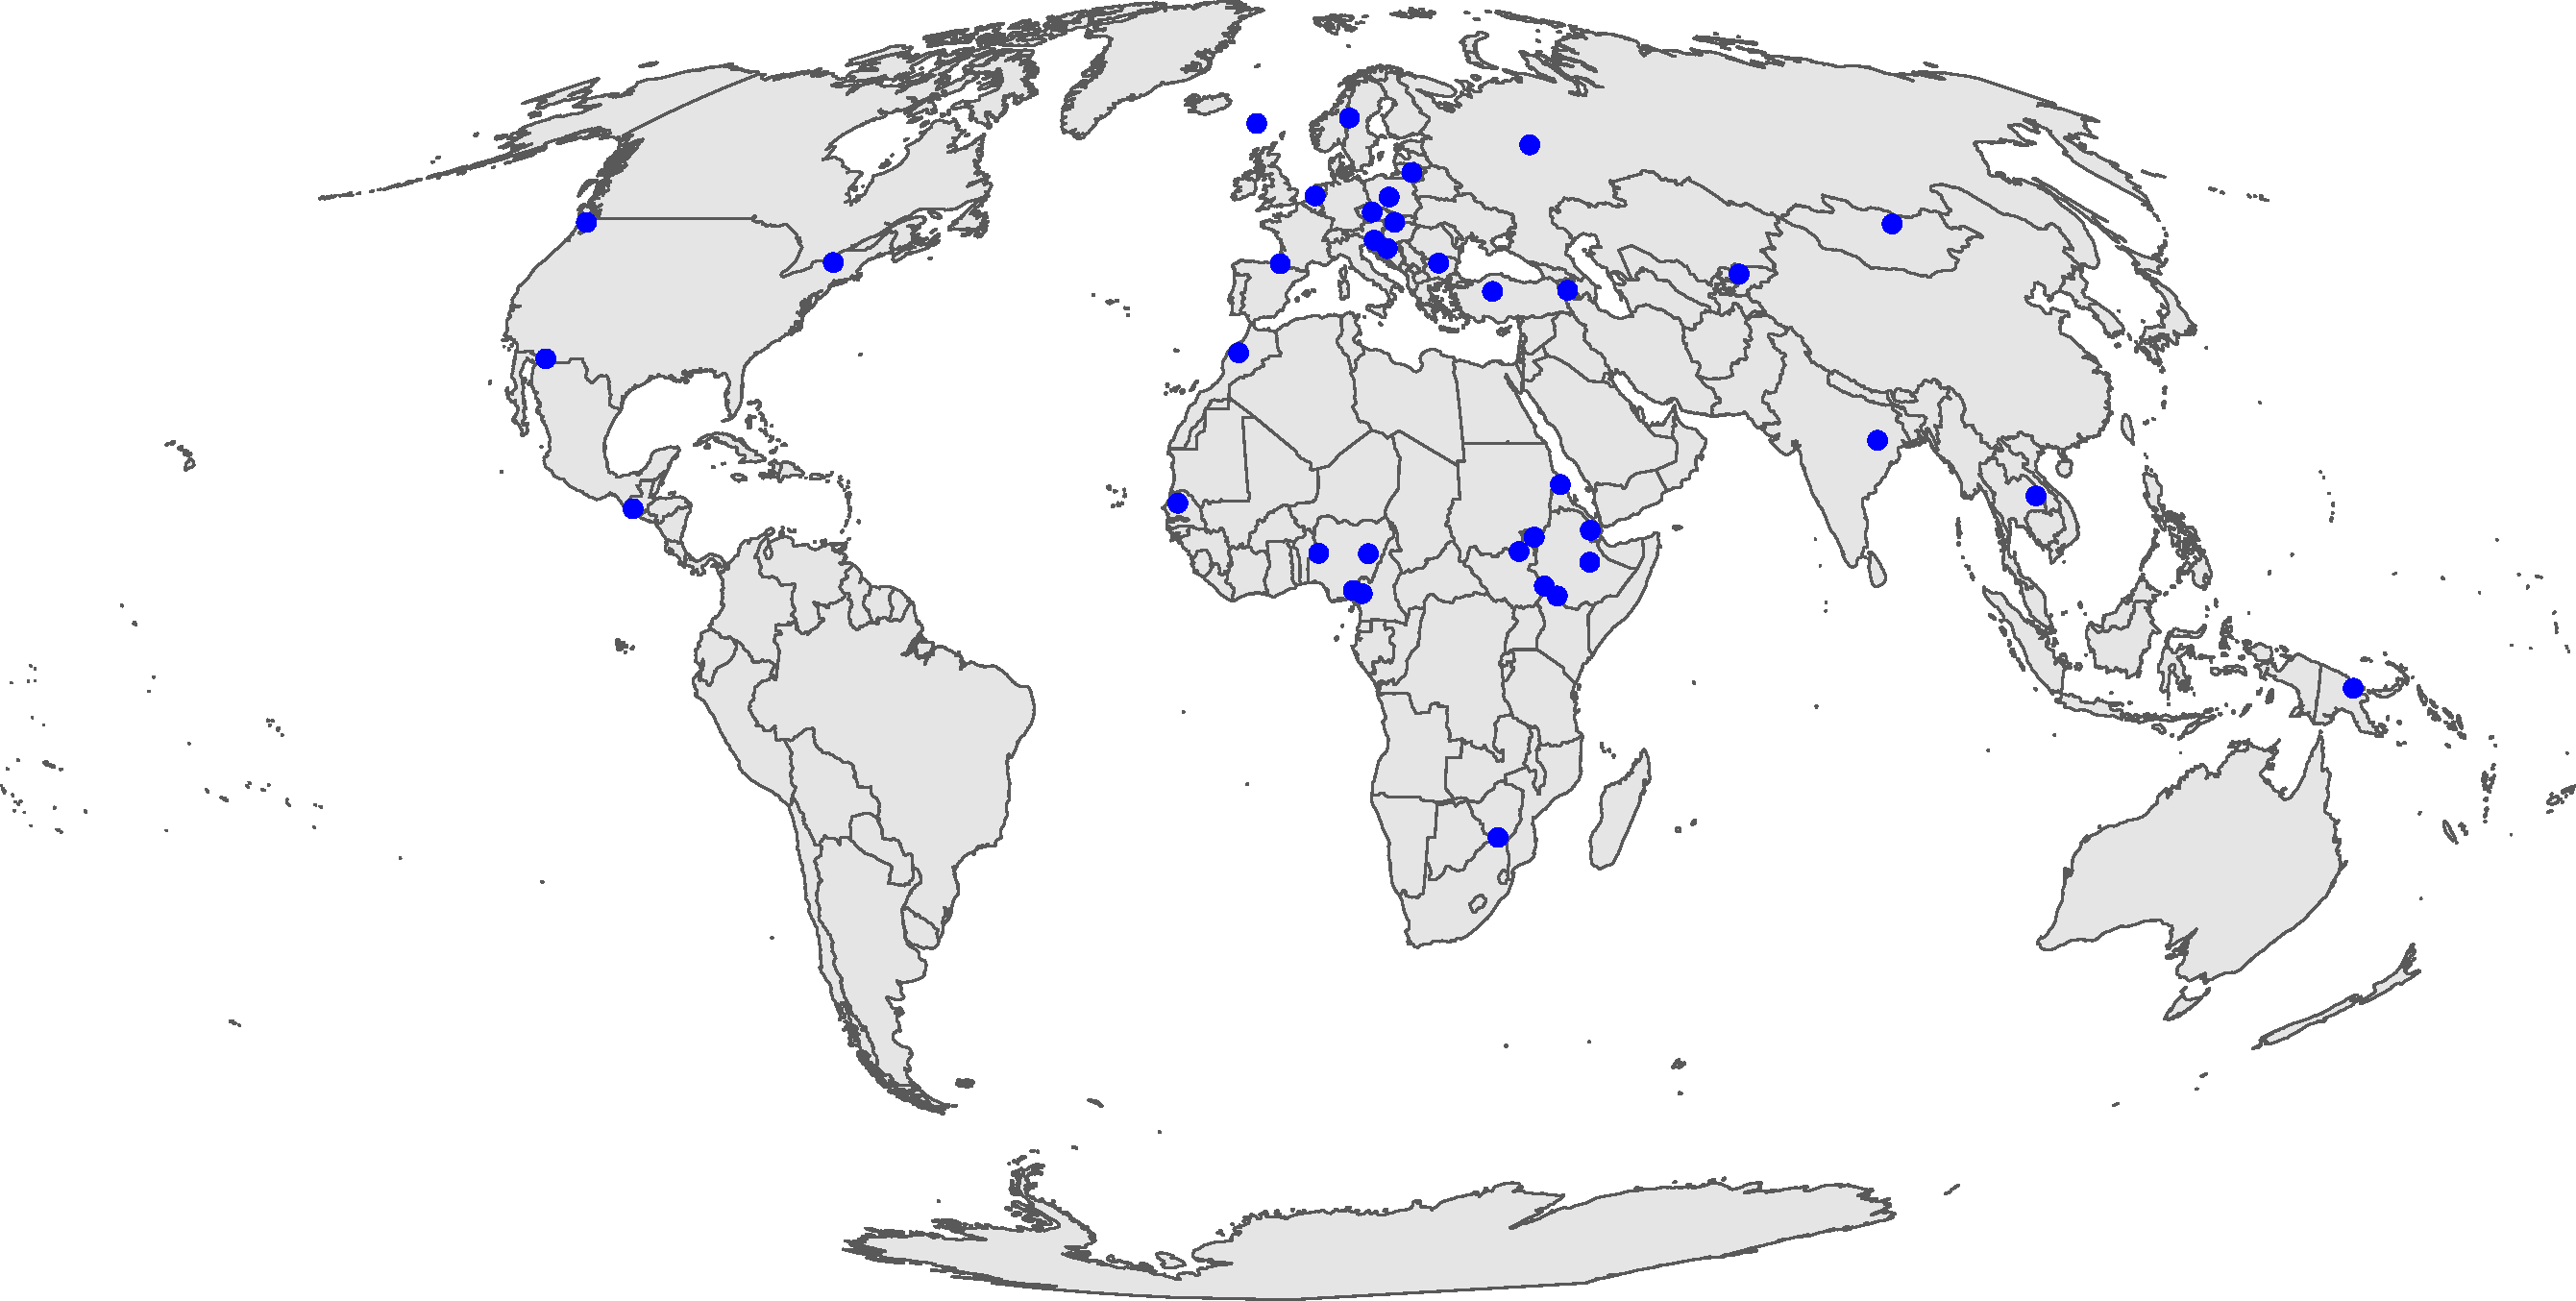
\includegraphics[width=\linewidth]{figures/final-devoicing.pdf}
\end{figure}

The picture shown in \figref{fig:final-devoicing} is, perhaps, rather surprising. Some version of final devoicing is found on most continents, but no examples are identified in Australia or South America: final devoicing is not rare, but neither is it ubiquitous. Perhaps even more surprisingly, in this presentation we see a rather pronounced areal signal: instances of this process appear to cluster especially strongly in Europe and in Ethiopia. Admittedly, both of these zones have been discussed as potential linguistic areas: cf. \textcite{könig1999sprachbund} on Europe and \textcite{ferguson1976ethiopian} on Ethiopia \parencite[but see the contrary view in][]{tosco2000is}. Even so, final devoicing is, to my knowledge, rarely pinpointed as potentially contributing to the definition of linguistic areas. For example, it is absent in \posscitet{ferguson1976ethiopian} list of possible phonetic traits of the Ethiopian area, whilst \textcite{ternes2010phonetische} provides a discussion of final devoicing in Europe but does not claim it as a \enquote{Europeme} (a feature that is exclusive to Europe or highly characteristic of it).

Of course, we should not take these findings too seriously. For one thing, given its  methods and aims, P-base is not even intended to present either a comprehensive view of phonological processes or a representative database addressing classical typological concerns of sampling bias \parencite[47--48]{mielke-diss}. Even a cursory glance at \figref{fig:final-devoicing} shows that, for instance, the Turkic languages, a genus where final devoicing is ubiquitous \parencite[27--28]{johanson2021structure}, are underrepresented in the data; the same applies to Austronesian, a phylum where final obstruent devoicing is rare as an alternation, but frequent as a sound change and (consequently?) a phonotactic restriction \parencite[\ppno~220--222, 246--247]{blust2013austronesian}. There is, of course, also an overall documentation bias: the kind of detailed data necessary to make inferences about  phonological patterns is simply more available for some languages compared to others, leading to underrepresentation of minoritized and indigenous languages. Furthermore, simple counting of attestations of a contextually restricted process such as final devoicing can never give a correct picture without controlling for phonotactic patterns or the presence of other phonological processes. Thus, no inference can be drawn from the absence of final devoicing in languages that do not permit any coda consonants at all, or where final consonants are subject to other processes (such as the neutralization of all word-final stops to \ipa{[ʔ]}, which is common, for instance, in Austronesian languages; \citealt[246--247]{blust2013austronesian}).

Nevertheless, this result should also give us pause. In particular, is the common intuition that final devoicing is frequent too reliant on the fact that it is (unusually?) common in familiar European languages? A salutary reminder here comes from \textcite{ladd2022mid}, who observes that phonological theories developed in Central and Western Europe, including Prague School structuralism, were very concerned with the question of neutralization, with the final devoicing of German, Russian, or Czech taking centre stage. Conversely, North America was dominated by \enquote{post\hyp Bloomfieldian} structuralism, whose \textit{lingua franca} was English, a language with very few neutralizing alternations of a similar kind\dash with the result that neutralization did not play an especially important role in the theory.

The central question of this chapter is how we can make progress towards a phonological typology that allows us to address the question of whether a particular phenomenon is rare (or, indeed, common) with the degree of rigour expected in modern typological enquiry. At first glance, phonology and phonetics should be amenable to the creation of empirically rich databases. Indeed, a priori we might expect this domain to be particularly well suited to the enterprise: relevant data is found in abundance both in broader typological databases such as WALS and in an increasing number of dedicated sources, with different sampling methods, coverage, and inclusion criteria, such as UPSID/LAPSyD \parencite{maddieson84:_patter,maddieson89:_updat_upsid, maddieson2013demonstration}, P-base \parencite{mielke-diss}, or PHOIBLE \parencite{phoible}, to name just a few, in addition to domain-specific databases such as BDPROTO \parencite{Moran2020}.

What kind of data do we find in these sources, and what kinds of research questions do they allow us to answer? First and foremost, they have tended to concentrate on phonemic inventories. In more senses than one, this is low-hanging fruit. The data is often easily available: most grammatical descriptions will include at least a phoneme chart, even if there is no other detailed phonological information. Second, phonemic inventories might seem particularly suitable for cross-linguistic comparison. After all, criteria for phonemic status appear to be widely agreed, uncontroversial, and applicable without much difficulty to most, if not all, languages across genealogical groupings and time periods and even modalities \parencite[see, however,][]{kiparsky2017formal}.

Indeed, we can point to some very real results and advances in a spatially and temporally embedded phonological typology, such as the demonstration of subtle and interesting areal signals in the distribution of affricates within Eurasia by \textcite{nikolaev2018areal} or the nuanced study of areal phonetics and phonology in the Caucasus by \textcite{grawunder2017caucasus}. The distributional typology of phonological inventories in segmental and suprasegmental domains has also informed other kinds of (often historically oriented) enquiry \parencite[e.\,g.][]{Atkinson2011,everett2013evidence,everett2015climate,Urban2021}.

As with other areas of typology, further advances are on the horizon. For instance,  \textcite{Nikolaev2019} offers the beginnings of a general theory of how language contact and areality can be reflected in distributional typology; \textcite{MacklinCordes2021} demonstrate how quantitative methods in the modelling of phonotactics can make further contributions to answering \enquote{what's where why} questions, while \textcite{napoleão2023beyond} extend typological methods to the domain of suprasegmental phonology; and \textcite{round2021historical} offer a quantitative approach to the long\hyp standing hypothesis that pathways of phonological change relate to the functional load of phonemic contrasts. Without wishing in any way to underplay the importance and significance of work already carried out on applying typological and/or phylogenetic methods to phonological systems, in this chapter I would like to address some key areas where \enquote{modern} phonological typology and considerations rooted in earlier approaches are in danger of becoming disconnected in ways that hinder further progress. In particular, I am concerned with the question of how much distributional typology can afford to abstract away from phonological theory. To put it another way: are the kinds of things phonologists are preoccupied with of any use to those working in typology? And if not, is it because phonologists have simply neglected something they should (also) work on, or are there issues that typologists need to engage with in order to reach a better understanding of the key questions of \enquote{what, where, when, and why}?

Like the problem of final devoicing, the case studies I use as a lens for addressing these issues are related to the phonology and phonetics of laryngeal contrast. In the next section, I discuss the typology of apparently simple, two\hyp way systems of laryngeal contrast and how it can be investigated using data on phonemic inventories.


\section{Levels of representation in phonological typology}
\label{sec:levels-representation}

In the earlier discussion of final devoicing in Friulian in \cref{typology-in-phonology} I referred to segments usually transcribed with symbols such as <d> as \enquote{voiced}, and those usually written as <t> as \enquote{voiceless}. However, we also noted that languages differ in the phonological content\dash the featural specification\dash of these labels, and consequently in the nature of final laryngeal neutralization \parencite{vaux05, iverson11:_final}. Equally, it is also well known that languages differ in the precise phonetic realization of the two categories \parencite[see, for instance][]{petrova06:_voice, chodroff2019covariation}. 

\textcite{Natvig2019}, building on \textcite{purnell2015distinctive}, offers a useful handle on understanding this variability. His discussion is focused on contact\hyp induced change, but the architecture is widely applicable. He distinguishes three levels of representation:

\begin{description}
\item [phonological:] inhabited by abstract categories implementing lexical contrasts; 
\item [phonetic-phonological:] where phonological categories are fleshed out in coarse phonetic detail, for example by specifying what kind of gestures (or more precisely \enquote{dimensions}, following \citealt{avery01:_laryn}) are involved;
\item [phonetic:] having to do with the language-specific implementation of the phonetic\hyp phonological representations, such as the specific timing of the gestures.
\end{description}

It can be shown that these levels are autonomous because we can identify cross\hyp linguistic variation in each of them. \textcite{Natvig2019} shows this with respect to how laryngeal phonology is affected in different contact settings, but this can also be demonstrated in more focused synchronic analyses: see, for instance, \textcite{honeybone05} on phonological variation, \textcite{avery01:_laryn} on phonetic\hyp phonological architecture, and any number of detailed studies of finely grained phonetic variation \parencite[on English laryngeal systems, see, for example][]{docherty92:_britis_englis,scobbie06:_flexib_englis_vot,Jacewicz2009,docherty14:_languag_scott_englis,Sonderegger2020}.

In this chapter, I will use this framework in concert with the \emph{amphichronic} approach, as developed by \textcite{bermudez-diachr, bermúdez-otero2015amphichronic, rbo2012cycles}. It assumes a view of phonological architecture that also distinguishes between the phonological grammar (a set of rules manipulating discrete representations) and the wider phonetic\hyp phonological system of the language that also comprises a set of \enquote{phonetic rules} regulating how phonological representations are implemented. The former maps neatly to the phonological level, whilst the latter broadly corresponds to the phonetic\hyp phonological and phonetic levels. A crucial notion is the \emph{life cycle of phonological processes}. Under this view, sound patterns arise out of the pool of acoustic and articulatory variation that exists primarily by virtue of non\hyp cognitive factors. First, they undergo the process of \emph{phonologization}, in which they become language\hyp specific phonetic rules, and later \emph{stabilization} as they enter the phonological grammar. \Cref{tab:levels-lifecycle} shows the mapping between the levels and notions related to the life cycle.

\begin{table}
  \centering
  \caption{Levels of representation and the life cycle}
  \label{tab:levels-lifecycle}
  \begin{tabularx}{\linewidth}{Q  QQQ}
    \lsptoprule
    Level             & Representations                              & Status of pattern            & Life cycle stage \\
    \midrule
                      & Acoustic events & Not under cognitive control & Pre-life cycle \\
    \midrule
    Phonetic & Gestural scores\ldots & \multirow[c]{2}{\Xhsize}[-.5\baselineskip]{Phonetic rule} & \multirow[c]{2}{\Xhsize}{Phonologization} \\
    \cmidrule{1-2}
    Phonetic-phonological & Dimensions\ldots & & \\
    \midrule
                            Phonological & Segments, features, metrical structure\ldots & Phonological rule & Stabilization    \\
    \lspbottomrule
  \end{tabularx}
\end{table}


This raises both conceptual and empirical questions. Conceptually, which, if any, of these levels is the right one for typological enquiry? The empirical question is perhaps more pressing: what data do the existing sources actually contain?

The most obvious answer is that this is the phonological level, which distinguishes a very limited number of \enquote{phonemic} series, such as {\VOICELESS} /p,~t,~k/ and {\VOICED} /b,~d,~ɡ/ in most languages of Western Europe. But what is the exact content of the units at this level, and how do we compare them across languages?

\subsection{Laryngeal specification and phonological contrast}
\label{sec:laryng-spec-contr}

We can start approaching this issue by considering inventories with only a single laryngeal series of obstruents. The typological import of such systems is discussed by \textcite{hyman08:_univer}. That paper, in offering detailed consideration of phonological typology from a more traditional perspective focused on language universals, raises precisely the question of the extent of analytic input into the construction of phonological \enquote{facts}. As \textcite{hyman08:_univer} discusses,  \enquote{all languages have [phonemic] voiceless stops} is a candidate for an absolute phonological universal, but its status hinges on the exact content of the label \enquote{voiceless}. He considers the status of languages such as Yidiɲ (\glottocode{yidi1250}, Pama-Nyungan~> Yimidhirr\hyp Yalanji\hyp Yidinic), which have a single series of stops that are realized with some degree of voicing. Do they falsify the universal? If we take the definition of \enquote{voiceless} to embrace phonetic detail, then Yidiɲ is clearly a counterexample. On the other hand, it is also possible to say, as \textcite{hyman08:_univer} does, that such a language has a single {\VOICELESS} series, if we take the observed phonetic voicing to be redundant, and irrelevant for our view of the phonological system. In this section, I expand on \posscitet{hyman08:_univer} point that typological generalizations in phonology can be difficult to even formulate, let alone verify, without reference to some theory of featural structure; see also \textcite{vaux2009, dresher2018contrastive, youssef2021contrastive} for recent restatements of the importance of attention to features in phonological typology.

Such theoretical questions are difficult enough to answer even \emph{a~priori}, without turning our attention to the quality of the underlying descriptions, and the role of variation in phonological analysis. How does the potentially \enquote{redundant} voicing in Yidiɲ stops compare with voicing in systems with a contrastive {\VOICED} series? More generally, how much variation can we allow: if we treat all languages without a laryngeal contrast as having a single {\VOICELESS} series, how much leeway can we give the phonetic component?

\textcite{kakadelis2018phonetic} offers some progress via a careful phonetic study of three such languages: Bardi (\glottocode{bard1255}, Nyulnyulan), Arapaho (\glottocode{arap1274}, Algic~> Algonquian), and Sierra Norte de Puebla Nahuatl (\glottocode{high1278}, Uto-Aztecan~> Aztec). She shows that despite the similarities in their phonology\dash they seem to have the same structure of laryngeal contrast\dash such systems implement the contrast very differently, in terms of timing, phonation, manner, and no doubt other properties. Kakadelis suggests that these findings \enquote{do not lend themselves to an analysis where \textins{the languages} share the same underlying laryngeal representation} (p.~290), implicitly rejecting analyses such as Hyman’s \parencite*{hyman08:_univer}. However, this conclusion only follows under certain theoretical premises, namely that the lack of laryngeal contrast \emph{within} the set of obstruents necessarily implies the lack of a phonological specification for laryngeal features. \textcite{kakadelis2018phonetic} suggests an analysis where privative features are assigned without regard to contrast, preserving the link between lack of phonological specification and increased range of phonetic variation, but at the cost of denying that contrast is important for featural structure.

However, depending on one’s theoretical commitments this difficulty is not insurmountable. The key issue here is the definition of \enquote{redundancy}. A key insight in phonology, going back all the way back to the Prague School, is that languages can differ in how \enquote{the same} phonetic substance is reified in terms of phonological contrast. This view is reiterated, for instance, by \textcite{lass1984vowel,simpson99:_fundam,vaux2009}.\footnote{See \textcite{trubetzkoy1931phonologie} for an early statement of this approach to the cross-linguistic comparison of phonological systems within a phoneme-based framework.} A prominent modern formalization of this approach is Modified Contrastive Specification \parencite{dresher09}. In this framework, it is perfectly possible to assign different featural specifications to superficially similar sets of segments without abandoning the commitment to avoiding redundancy in featural structure. Crucially, this approach makes specific predictions relating the place of laryngeal features within the contrastive hierarchy and patterns of phonetic underspecification and variation, which we can test against the observed systems.\footnote{For extended concrete applications of the approach linking contrastive feature scope and phonetic variation, see recently \textcite{dresher2018contrastive, natvig2018contrast,Purnell2019}.}

Let us first consider a system like Bardi \parencite{Bowern2012,kakadelis2018phonetic}, an indigenous Australian language not dissimilar to Yidiɲ. Here, \enquote{stops} show extensive variation in terms of both voicing and manner. Within the consonant inventory, the \enquote{stops}\dash the label is something of a misnomer, given the ubiquity of a lenition process that often results in continuant articulations\dash contrast with nasals, laterals, rhotics, and glides. By contrast, all the sonorants are described as \enquote{phonetically and phonologically stable segments} by \textcite[339]{Bowern2012}. We can analyse the inventory of Bardi with wide scope for the manner features corresponding to nasality, laterality, and rhotic status, as sketched in \figref{fig:bardi-ch}.\footnote{For concreteness, I use an abstract \enquote{cover} feature for \enquote{rhotic manner}. I also use binary features here, but a privative system is, if anything, more suited to capturing the kind of underspecification insights the analysis seeks to capture. See \textcite{currie07,iosad2017phonologization,sandstedt2018feature} for approaches combining privative features with Modified Contrastive Specification.} The lack of obstruent specification (and \emph{a fortiori} laryngeal specification) accounts for the unstable behaviour of the segments in question.

\begin{figure}
\centering
\caption{An outline contrastive hierarchy for Bardi}
\label{fig:bardi-ch}
\begin{forest}for tree={align=center}
  [p t ʈ c k m n ɳ ɲ ŋ l ɭ ʎ r ɻ\\ {\mbox{[±nas]}}
    [p t ʈ c k l ɭ ʎ r ɻ\\ {\mbox{[±lat]}}, minus
      [p t ʈ c k r ɻ\\ {[$\pm$rhotic]}, minus
        [p t ʈ c k\\ Place\ldots, minus]
        [r ɻ\\ Place\ldots, plus]]
      [l ɭ ʎ\\ Place\ldots, plus]]
    [m n ɳ ɲ ŋ\\ Place\ldots, plus]
  ]
\end{forest}
\end{figure}

In Sierra Norte de Puebla Nahuatl, the stops \ipa{/p,~t,~k,~kʷ/} are generally voiceless, albeit with a significant proportion of closure voicing in contexts where phonation (modal voicing) typically perseveres from the preceding context (intervocalically and especially after a nasal). Unlike Bardi, they are not especially prone to lenition, with the exception of the velars, which are often realized with voicing and/or as continuants. This may have led to the appearance of a phonemic \ipa{/ɣ/}, which is nevertheless highly marginal. This system can be accommodated if velars are specified for neither voicing nor continuancy, whilst the other stops are contrastively noncontinuant, but still underspecified for voicing. One contrastive hierarchy that meets this requirement is shown in \figref{fig:snp-nahuatl-ch}. Here, the place feature for velars takes scope over the manner features that come into play for other stops, rendering them redundant in the velar subinvenory. This results in a high degree of underspecification similar to what we saw in Bardi. The other stops do enter a manner contrast with fricatives: this motivates a categorical specification as noncontinuants, accounting for their resistance to lenition. However, there is no need to set up a voice contrast for these segments, which leaves some leeway for variation in this dimension.


\begin{figure}
  \caption{An outline contrastive hierarchy for Sierra Norte de Puebla Nahuatl}
  \label{fig:snp-nahuatl-ch}
  \begin{forest}
    [p t k kʷ s ʃ t͡s t͡ʃ l n m w j\\\mbox{[±sonorant]}
      [p t k kʷ s ʃ t͡s t͡ʃ\\\mbox{[±back]}, minus
        [p t s ʃ t͡s t͡ʃ\\\mbox{[±continuant]},minus
          [p t t͡s t͡ʃ\\\mbox{[±strident]}, minus
            [p t\\Place\ldots,minus]
            [t͡s t͡ʃ\\Place\ldots,plus]]
          [s ʃ\\Place\ldots, plus]]
        [k kʷ\\Place\ldots,plus]]
        [l m n w j\\{Manner, Place\ldots}, plus]]
  \end{forest}
\end{figure}


Finally, in Arapaho the apparently {\VOICELESS} stops also fall into two classes. The non\hyp labial stops are relatively stable in terms of both manner and phonation-related properties such as VOT. Like in Sierra Norte de Puebla Nahuatl, stops at non\hyp labial places of articulation contrast with a series of fricatives, which contributes to the lack of variation in manner. In this language, it is the labial stop that both lacks a fricative counterpart and is significantly more prone to both manner lenition and voicing. The difference, however, is that these stops also resist closure voicing, suggesting they are contrastively {\VOICELESS}. An analysis reflecting these specifications is sketched in \figref{fig:arapaho-ch}.

\begin{figure}
\centering
\caption{An outline contrastive hierarchy for Arapaho}
\label{fig:arapaho-ch}
\begin{forest}for tree={align=center}
  [n p t t͡ʃ k ʔ θ s x h j w\\ {\mbox{[±rd]}}
    [n t t͡ʃ k ʔ θ s x h j\\ {\mbox{[±voi]}}, minus
      [t t͡ʃ k ʔ θ s x h\\ {\mbox{[±cont]}}, minus
        [t t͡ʃ k ʔ\\ Place\ldots, minus]
        [θ s x h\\ Place\ldots, plus]]
      [n j \\ Manner\ldots, plus]]
    [p w\\ Manner\ldots, plus]
  ]
\end{forest}
\end{figure}

\subsection{Laryngeal contrast and phonetic-phonological variation}
\label{sec:laryng-contr-phon}

The discussion in \cref{sec:laryng-spec-contr} aimed to demonstrate the existence of a non\hyp trivial space of possibilities available to encode sparse phonological representations that lack a lot of the phonetic detail in the construction of typological datasets. The challenges become even more acute if more descriptive phonetic detail is admitted into the typology. Consider a simple two-term system distinguishing a {\VOICELESS} and a {\VOICED} series. There is an extensive literature claiming that such a pattern of phonological contrast can be implemented in multiple ways \parencite[cf.][]{beckmanng:_empir, salmons2017germanic}. Generally, {\VOICELESS} stops can be realized with short-lag voice onset time (\enquote{voiceless unaspirated}) or with long\hyp lag VOT (\enquote{voiceless aspirated}), whilst {\VOICED} stops run the gamut from consistently prevoiced (VOT lead) in all positions to consistently voiceless (unaspirated), with many languages showing extensive surface variability.

To probe this variation, \cref{tab:laryngeal-contrasts} lists some languages for which this issue has been addressed in the phonetic literature, grouped into four broad \enquote{types}, and compares the results to the listing in PHOIBLE \parencite{phoible}. Where PHOIBLE includes more than one entry for a particular language, or records synchronic variation, I use the $\sim$ symbol to record the variants. (To save space, I do not distinguish between the two possibilities.) The \enquote{types} are, broadly, \enquote{voicing} languages with no aspiration in the {\VOICELESS} series and consistent prevoicing of {\VOICED} stops; \enquote{aspirating} languages contrasting aspirated and variably voiced series; \enquote{voiceless} languages where both {\VOICELESS} and {\VOICED} stops are realized without vocal fold vibration; and \enquote{overspecified} languages in which both aspiration and prevoicing are consistently used in the respective series.\footnote{The sources used are as follows: Russian \glottocode{rus1263} \parencite{ringen2012voicing}, French \glottocode{stan1290} \parencite{abdelli-beruh2004stop}, English \glottocode{stan1293} \parencite{jansen07:_phonol_englis}, German \glottocode{stan1295} \parencite{jessen02:_laryn_german}, Turkish \glottocode{anat1259} \parencite{kallestinova04:_voice_turkis}, Persian \glottocode{west2369} \parencite{bijankhan2009voice}, Scottish Gaelic \glottocode{scot1245} \parencite{Nance2019}, Danish \glottocode{dani1285} \parencite{hutters85:_vocal_danis, puggaard-rode2022danish}, Ulster Irish \glottocode{done1238} \parencite{nichasaide1986preaspiration}, Swedish \glottocode{stan1279} \parencite{helgason08:_voicin_swedis}, Najdi Arabic \glottocode{najd1235} \parencite{al-gamdi2019najdi}, Mehri \glottocode{mehr1241} \parencite{Watson2016}. None of the sources listed here appear in the bibliography for PHOIBLE, although I have not excluded the possibility that some of PHOIBLE's sources may in turn rely on these.}

\begin{sidewaystable}
  \begin{threeparttable}
  \caption{Some systems of laryngeal contrast}
  \label{tab:laryngeal-contrasts}
  \begin{tabularx}{.85\textheight}{Xlcccc}
    \lsptoprule
                      &                       & \multicolumn{2}{c}{Source} & \multicolumn{2}{c}{PHOIBLE}                          \\
    \cmidrule(r){3-4} \cmidrule(l){5-6}
    Type              & Language              & {\VOICELESS}                  & {\VOICED}                     & {\VOICELESS}      & {\VOICED} \\
    \midrule
    Voicing           & Russian         & p, t, k                      & b, d, ɡ                      & p, t, k          & b, d, ɡ  \\
                      & French           & p, t, k                      & b, d, ɡ                      & p, t, k          & b, d, ɡ  \\
    \midrule
    Aspirating        & English          & pʰ, tʰ, kʰ                   & b$\sim$b̥, d$\sim$d̥, ɡ$\sim$ɡ̊ & pʰ, tʰ, kʰ       & b, d, ɡ  \\
                      & German           & pʰ, tʰ, kʰ                   & b$\sim$b̥, d$\sim$d̥, ɡ$\sim$ɡ̊ & p(ʰ), t(ʰ), k(ʰ) & b, d, ɡ  \\
                      & Turkish          & pʰ, tʰ, kʰ                   & b$\sim$b̥, d$\sim$d̥, ɡ$\sim$ɡ̊ & p(ʰ), t(ʰ), k(ʰ) & b, d, ɡ  \\
                      & Persian          & pʰ, tʰ, kʰ                   & b$\sim$b̥, d$\sim$d̥, ɡ$\sim$ɡ̊ & pʰ, tʰ, kʰ       & b, d, ɡ  \\
    \midrule
    \multirow[t]{3}{\hsize}{Voiceless} & Scottish Gaelic  & pʰ, tʰ, kʰ                   & p, t, k                      & pʰ, tʰ, kʰ       & p, t, k  \\
                      & Danish           & pʰ, tʰ, kʰ                   & p, t, k                      & 
                                      \begin{minipage}[c]{.18\textwidth}
                                        \centering \mbox{pʰ, t͡sʰ, kʰ $\sim$ b̥ʰ, d̥ʰ, ɡ̊ʰ}
                                      \end{minipage}
                      & b̥,  d̥,  ɡ̊ \\
                      & Ulster Irish     & pʰ, tʰ, kʰ                   & p, t, k\tnote{*}  & p, t, k & b, d, ɡ  \\
    \midrule
    Overspecified     & Swedish          & pʰ, tʰ, kʰ                   & b, d, ɡ                      & p(ʰ), t(ʰ), k(ʰ) & b, d, ɡ  \\
                      & Najdi Arabic     & tʰ, kʰ                      & b, d, ɡ                      & t, k            & b, d, ɡ  \\
                      & Mehri            & tʰ, kʰ                      & b, d, ɡ                      & tʰ, kʰ          & b, d, ɡ  \\
    \lspbottomrule
  \end{tabularx}
  \begin{tablenotes}
    \item [*] Some perseverative voicing
  \end{tablenotes}
\end{threeparttable}
\end{sidewaystable}


The point of this exercise is not to quibble about the quality of the PHOIBLE data: after all, it can only be as good as the available sources. Rather, it is to examine how the observed variation is encoded in a database. What \cref{tab:laryngeal-contrasts} shows is that the only type for which the relationship between the phonetic findings and the PHOIBLE encoding is consistent is the \enquote{voicing} class contrasting {\VOICELESS} [p,~t,~k] and fully voiced [b,~d,~ɡ]. In other cases, there is a degree of inconsistency as to whether aspiration is represented in the database, and the reflection of variable voicing in the {\VOICED} series appears to be a particular source of divergence.

Even allowing for the multiple representations found in the database, \cref{tab:laryngeal-contrasts} significantly underplays the synchronic degree of variation observed in the languages listed. Even the sparse encoding shown here brings across some aspects of its aspects, as in the very strong affrication of the {\VOICELESS} coronal stop \ipa{[tʰ]} (or \ipa{/t/}?) in Danish. Even a single parameter such as VOT will often show meaningful variation within a speech community, including social and geographical variation \parencite[cf. on Danish][]{puggaard2021jutlandic}, that is not easily captured by picking one, or even several, discrete transcription symbols. Importantly for the issue of levels of representation, extensive empirical work has demonstrated how patterns that can look superficially very similar can have very different aetiologies \parencite{pierrehumbert00:_concep,scobbie07:_inter}, sometimes even within the same speech community \parencite[for examples, see][]{myers-phonoknowledge,przezdziecki05:_vowel_yorub,strycharczuk2014phonetic}. In any case, VOT is only one parameter: whilst we have at least some understanding of the typological variation in this dimension \parencite{petrova06:_voice, chodroff2019covariation}, other phonetic cues such as duration, F0 perturbations, or the effect on neighbouring vowels remain grossly understudied from a cross\hyp linguistic perspective; cf. on laryngeal distinctions specifically \textcite{kirby2019effects} and on more phonetic microvariation more generally \textcite{anderson2018, heggarty_sound_2019}.

Even assuming we have the right data, however, which of the three levels of representation is a database of \enquote{phonemic inventories} meant to encode? How much variation do we include, and how do we represent it? For example, English, Danish, and Swedish, despite the different phonetics of laryngeal contrast, all show very similar patterns of morphophonological behaviour related to laryngeal features, in which the {\VOICELESS} series behaves as relatively marked (in a formal sense) and the {\VOICED} series is relatively unmarked.\footnote{\Textcite{iverson99:_laryn_german} offer extensive discussion of this analysis, which is widely, but far from universally, accepted. For a recent exposition of the dissenting view, see \textcite{ahmed2020english}.} Should we choose a phonetically sparse, abstract encoding reflecting the phonological level, with a {\VOICELESS} series (perhaps /p,~t,~k/) and a {\VOICED} one (/b,~d,~ɡ/?), identical to the system of Russian or French? Or perhaps we accept that it is the phonetic\hyp phonological level that is most relevant? In this case, aspiration in the {\VOICELESS} series would have some phonological significance, leading us to postulate different phonological representations of these types of laryngeal contrast. Such an approach \parencite[cf.][]{salmons2017germanic}  would allow us to reflect the phonological characteristics of such languages whilst effacing details (like the precise phonetics of the {\VOICED} series) that have no phonological import.

On the other hand, encoding redundant detail runs the risk of erasing differences that are not apparent from an examination of the more concrete phonetic characteristics of the pattern. For instance, as \cref{tab:laryngeal-contrasts} shows, voiceless unaspirated [p,~t,~k] stops realize the phonological {\VOICELESS} series in a \enquote{voicing} language like Russian but the phonological {\VOICED} series in a language like Ulster Irish (\glottocode{done1238}, Indo\hyp European~> Celtic).\footnote{This comparison is not entirely exact, as Ulster Irish {\VOICED} stops do show a degree of voicing in postvocalic position, interpreted by \textcite{nichasaide1986preaspiration} as passive (coarticulatory).} This is reflected in both their phonology and their language\hyp specific phonetics. For instance, phonologically {\VOICELESS} [p,~t,~k] stops have longer closure durations than the {\VOICED} series \parencite[for Russian, see e.\,g.][]{ringen2012voicing}, but when \ipa{[p,~t,~k]} are phonologically {\VOICED} the relationship is reversed, as in Ulster Irish \autocite[174]{nichasaide1986preaspiration}. Phonologically, [p,~t,~k] pattern as {\VOICELESS} in Russian, where they trigger assimilatory devoicing. In Ulster Irish, they alternate with {\VOICED} continuants under conditions of initial mutation,\footnote{In the same context, {\VOICELESS} [pʰ,~tʰ,~kʰ] alternate with {\VOICELESS} [f,~h,~x].} and coalesce with /h/ to produce the {\VOICELESS} stops \parencite{buachalla85:_moder_irish}. Given these circumstances, are the phones transcribed as [p,~t,~k] comparable across languages? Here, \textcite{Ladd_2014} provides some very pertinent criticism, focusing on the very notion of a \enquote{phone}, that addresses this point, which is itself of course also familiar as a broader concern in linguistic typology.

Possibly important as these considerations are, it could be argued that they miss the point. The purpose of distributional typology, after all, is not to offer in-depth individual case studies, but to uncover patterns and regularities on a larger scale (the \enquote{wood}, as it were) that are easy to miss, if at all possible to find, by an aggregation of individual analyses (the \enquote{trees}). Nevertheless, I suggest that these problems do matter, and progress in phonological typology depends on close engagement with them. In the next section, I discuss the typology of an alleged phonological rarity, namely {\VOICELESS} stop preaspiration, in light of these issues of phonological analysis.

\section{How rare is preaspiration, really? And why?}
\label{sec:how-rare-preasp}
\begin{sloppypar}
Preaspiration, which is usually seen as especially associated with {\VOICELESS} stops, is a phenomenon frequently cited as a phonological rarum: for detailed discussion, see \textcite{silverman03}, \textcitetv{chapters/16_Hejná}, and \textcitetv{chapters/17_Craioveanu}. The starting point for much research in the area has been, as so often, grounded in the situation found in the languages of Europe. Preaspiration appears to act as an areal feature in northern Europe, being found in at least three genetically diverse groups: (North) Germanic, (Goidelic) Celtic, and Finno-Ugric (specifically Sámi). Early discussions of this areal feature have consistently treated this phenomenon as cross\hyp linguistically very rare \parencite[e.\,g.][]{marstrander1932okklusiver, wagner1964nordeuropäische}, and although some surveys have turned up a range of parallels elsewhere \parencite{liberman84:_german, silverman03}, this view remains firmly established \parencite{salmons92:_accen, hansson2001remains, blevins2017areal}, despite some dissenting voices (\citealt{Clayton2010}, \citetv{chapters/17_Craioveanu}).
\end{sloppypar}

The basics of this view run as follows. Preaspiration of {\VOICELESS} stops is narrowly defined as a period of glottal friction associated with the oral closure, often with the qualification that an interpretation of this structure as a surface [hC] cluster is not desirable or convincing. Understood in this way, it appears cross-linguistically rare. The common explanation is that such preaspiration is perceptually weak, and therefore vulnerable to change, being either lost or, conversely, \enquote{strengthened} to an oral segment \parencite{silverman03}. However, in Northern Europe we find it in a group of unrelated languages that have historically been in contact. Unsurprisingly, then, proposals to derive its spread from language contact date back at least to \textcite{marstrander1932okklusiver}; discussions of this phenomenon specifically as an areal feature include \textcite{wagner1964nordeuropäische,borgstroem74,salmons92:_accen,eliasson2000typologiska,hansson2001remains,rießler2008substratsprachen,blevins2017areal}.

Since the alleged cross\hyp linguistic rarity of the phenomenon motivates much of this research, it is important to interrogate it: is preaspiration really rare? The answer to this questions depends both on how we define preaspiration, and on what the baseline for \enquote{rarity} is.

\subsection{Preaspiration and levels of representation}
\label{sec:preasp-levels-repr}

Here, I do not focus too much on the recent empirical findings that demonstrate how preaspiration is much more widely distributed cross\hyp linguistically than previously appreciated; I refer to \textcitetv{chapters/16_Hejná} and \textcitetv{chapters/17_Craioveanu} for more in-depth discussion. Granting that preaspiration is not as much of a \emph{rarissimum}, what can we say about its precise representation?

\textcitetv{chapters/17_Craioveanu} defends a maximalist approach, in which all instances of preaspiration are treated as instances of a coda \ipa{[h]} segment; in terms of the three levels of representation, this is clearly a fact that belongs to the phonology. I see no reason to doubt that phonological preaspiration of this nature does exist. Icelandic (\glottocode{icel1247}, Indo-European~> Germanic) is probably by far the best\hyp known case (see \citealt{árnason2011icelandic}: §11.2 for a review of the evidence that Icelandic preaspiration is best treated as a coda segment), but others also exist. Northern Sámi (\glottocode{nort2671}, Uralic~> Saami) provides a pertinent example \parencite{sammallahti1998saami, sammallahti2019láidehus, bye2001virtual, aikio2022north}. In general, the language distinguishes two varieties of preaspirated stops (and affricates). Within the overall quantity system, they are equivalent to long and overlong varieties of other consonants (also referred to as \enquote{short geminates} vs. \enquote{long geminates}): the relationship of forms like \textit{lahki} `half.\Gen.\Sg' and \textit{lahkki} `half.\Nom.\Sg' is parallel to that between \textit{guossi} `guest.\Gen.\Sg' (with long \ipa{[sː]}) and \textit{guos\textquotesingle si} `guest.\Nom.\Sg' (with overlong \ipa{[sːs]}). These segments alternate with each other as part of an elaborate morphophonological pattern known as \emph{consonant gradation}, in which both individual consonants and consonant clusters appear in one of two shapes, referred to as the \enquote{strong} and \enquote{weak} grades \parencite[for an overview, see][]{bakró-nagy2022consonant}.

The realization of the contrast between the two series differs across dialects. In many Sea Sámi varieties, such as that of Maattivuono \parencite[17--18]{ravila1932}, the difference lies primarily in the duration of the stop closure, with the preaspiration described as very short. In Western Inland dialects, such as those of Western Finnmark or Eastern Eanodat (Enontekiö), the difference between the two lies in the duration of the preaspiration instead: short \ipa{[lɑhkiː]} for \textit{lahki} `half.\Gen.\Sg' vs. long \ipa{[lɑhːkiː]} \textit{lahkki} `half.\Nom.\Sg' \parencite[130]{sammallahti2019láidehus}.\footnote{The exact transcriptions in the source, which uses a version of the Finno-Ugric Phonetic Transcription, are <la˙hkii> and <la˙h.ʰ.kii> respectively, where the raised dot indicates stress, and the full stops refer to \enquote{glottal pulses}.} This, by itself, does not guarantee the segmental status of preaspiration, but the patterns of Eastern Inland dialects such as those of the Deatnu (Tana) river valley, are more probative. Here, the two kinds of stops do not differ in the duration of preaspiration, which is always short. Indeed, in certain varieties (e.\,g. Upper Deatnu) distinctions such as those between \textit{rohkki} `dead person.\Nom.\Sg' and \textit{rohki} `dead person.\Gen.\Sg' are neutralized in favour of the short preaspiration, with both being realized as \ipa{[rohkiː]} \parencite[141]{sammallahti2019láidehus}. In others (e.\,g. Veahčat), however, the difference is maintained thanks to the fact that the preceding vowel is long before the expected short preaspiration \textit{áhčči} `father.\Nom.\Sg' \ipa{[æht͡ʃiː]} vs. \textit{áhči} `father.\Gen.\Sg' \ipa{[æːht͡ʃiː]} \parencite[163]{sammallahti2019láidehus}. I suggest that this variation is best understood if we accept that the preaspiration \ipa{[h]} is, or in some varieties was at the earlier stage, a segment carrying distinctive quantity.

\largerpage
\begin{sloppypar}
The segmental status of \ipa{[h]} is supported because its patterning parallels quite precisely the behaviour of the first member in a continuant\hyp consonant cluster. In particular, consonant gradation in fricative\hyp initial clusters like those in \textit{niski} `nape', show the same patterns as that involving preaspirated stops (quantity distinction in the first consonant in Western Inland; neutralization or vowel quantity distinction in Eastern Inland). \Textcite{bals2006north, bals2012north} describe and analyse the Western Inland dialect of Guovdageaidnu, where the distinction between short and long preaspiration coexists with vowel lengthening before the short version to produce pairs like \ipa{[ahːt͡ʃi]} `father.\Nom.\Sg', weak grade \ipa{[aːht͡ʃi]} `father.\Gen.\Sg'. They analyse this pattern via a rule of Pre-Continuant Lengthening, which applies in the \enquote{weak grade} not only before preaspiration but also before other continuants. The rule applies before short geminate consonants (\textit{golli} `gold.\Gen.\Sg' \ipa{[koːlːi]}) and consonant clusters (\textit{niskki} `nape.\Gen.\Sg' \ipa{[niːski]}); contrast with unlengthened \textit{gol\textquotesingle li} `gold.\Nom.\Sg' \ipa{[kolːli]}, \textit{niski} `nape.\Nom.\Sg' \ipa{[nisːki]}.  Crucially, the weak grade alone is not a sufficient condition for lengthening: vowels remains short before weak\hyp grade stops (in items like \textit{loddi} `bird.\Nom.\Sg', weak grade \textit{lotti}). In other words, \enquote{\ipa{[h]} + stop} sequences pattern with continuant geminates and continuant\hyp initial clusters, and not with geminate unaspirated stops, strongly suggesting that \ipa{[h]} is a continuant segment.

Similar facts obtain in dialects like Deatnu Valley. They lack quantitative distinctions between short and long preaspiration, as well as between strong and weak grades of continuant geminates and clusters like \textit{sk}. However, this cannot be ascribed to a general neutralization of the grade alternation, because the weak grades remain distinct in other cases, especially where the contrast is also expressed by the duration of the second consonant: \textit{čalbmi} `eye.\Nom.\Sg' with \ipa{[lm]} vs. \textit{čalmmi} `eye.\Gen.\Sg' with \ipa{[lmː]} \parencite[141]{sammallahti2019láidehus}. Thus, also in these dialects \enquote{preaspirated stops} specifically pattern like continuant geminates and continuant\hyp initial clusters, but not like stops.
\end{sloppypar}

\largerpage
Dialects like Upper Deatnu provide further evidence that this phenomenon cannot be due to relatively low\hyp level phonetic timing processes related to metrical contrasts \parencite[cf.][]{hiovain2020dialectal}, but has undergone stabilization and participates in segmental phonology. This is because some nuclei (particularly the historical opening diphthongs) show qualitative, rather than quantitative distinctions with a parallel distribution to how long and short vowels are sensitive to the status of preaspiration. In Veahčat, the qualitative distinctions may be accompanied by the maintenance of the quantitative contrast: hence \ipa{[rŏ͜æ̆hkiː]} \textit{roahkki} `hook.\Nom.\Sg' but \ipa{[ru͜æhkiːh]} \textit{roahkit} `hook.\Nom.\Pl'. In Upper Deatnu, however, the quantitative distinction is neutralized but the quality differences remain, producing the pair \ipa{[rŏ͜æ̆hkiː]} vs. \ipa{[rŭ͜ŏhkiːh]}  \parencite[65]{sammallahti2019láidehus}.\footnote{Strictly speaking, \textcite{sammallahti2019láidehus} suggests that the diphthongs also differ in the placement of stress within the diphthong, with notations like <ŭĕ˙> vs. <ŭ˙ŏ>. However, this \enquote{stress placement}, whatever its precise phonetic correlates, appears to be generally predictable from the quality and length of the diphthong.} The segmental distinctions in the diphthongs are synchronically opaque with regard to the quantity of the following segment, including the preaspiration, which strongly suggests the latter had been stabilized as part of the life cycle. Thus, there is considerable evidence for the segmental status of preaspiration in at least some varieties of Northern Sámi.

That being said, I suggest that phonological preaspiration is \emph{not} the only possibility. The occurrence of glottal friction before a stop closure can correspond to a phonological \ipa{[h]} segment, but it can also be a by\hyp product of the fact that the stop (usually of the {\VOICELESS} series) is associated with glottal spreading without such a segment being present in the surface phonological representation: preaspiration belongs to the phonetic-phonological level, in this case. If a language has a \enquote{phonetic rule} of preaspiration as part of how the abstract category of {\VOICELESS} is mapped to phonetic substance, it may very well show some language\hyp specific patterning in terms of duration or asymmetries in behaviour determined by factors such as consonant place. Such restrictions may very well be quite similar to those visible in the behaviour of preaspiration that has been stabilized (in the life cycle sense), which exists at the phonological level. However, the root cause of this is not some fundamental identity between the two, but rather their diachronic relationship: within the architecture of the life cycle of phonological patterns, phonological preaspiration rules arise from phonetic ones.

Distinguishing between the two kinds of preaspiration is not at all trivial. I refer to \textcite{iosad2020phonological} for more detailed discussion. The most important consideration here is the fundamental criterion we should use to draw this line. Much of the recent work in the field builds on \posscitet{helgason} distinction between \enquote{normative} (obligatory, categorical) and non\hyp normative (non\hyp obligatory, variable) preaspiration \parencite[cf.][]{hansson2001remains, blevins2017areal}. However, like \textcitetv{chapters/17_Craioveanu} I believe this distinction does not map to an architecturally useful difference: there is certainly no guarantee that a phonological phenomenon cannot be variable \parencite{cohn06:_is, fruehwald2021oxhop}. Instead, I suggest that the defining criterion here is \emph{modularity} \parencite[cf.][]{iosad2017phonologization}. Phonological rules are categorical manipulations of discrete entities such as segments and other representations of the phonological level (for instance, pieces of autosegmental structure); phonetic rules take surface phonological representations and map them to real\hyp valued phonetic properties (as part of the phonetic-phonological and phonetic components).

This issue, which rides on whether preaspiration is represented in the phonological grammar of the language, is in principle orthogonal to the much\hyp discussed question of how laryngeal articulations such as aspiration and glottalization interact with segmental representations. There is a wealth of scholarship in theoretical phonology discussing the representation of laryngeally modified segments, including their possible nature as complex segments, the precise nature of any subsegmental structure necessary to represent relevant timing relationships, the rôle of factors such as sonority and metrical (syllabic) structure in the licensing and alignment of such articulations, and many others (in addition to \citetv{chapters/17_Craioveanu}, relatively recent discussions can be found in \cites{steriade1993segments}{howe2001patterns}{Davis2003}{kehrein04}{golston2013}). In particular, the critical issue of whether timing and alignment must be phonologically represented, as in Aperture Theory \parencite{steriade1993segments} or Q Theory \parencite{inkelas2017looking} or is up to the phonetic (or phonetic\hyp phonological, in our terms) component \parencite[e.\,g.][]{howe2001patterns} is both highly sensitive to background theoretical assumptions that we cannot treat in detail here and requires careful empirical underpinning, which for many relevant cases remains a desideratum. For now, I will set it aside, and focus on the central problem of architectural affiliation.

Under this régime, identifying whether a preaspiration rule is phonological or phonetic requires detailed analysis of each particular case. This also means that cross\hyp linguistic comparison, in and of itself, becomes much less probative. Consider the case of Faroese (\glottocode{faro1244}, Indo\hyp European~> Germanic), a close relative of Icelandic. The distribution of preaspiration in Faroese is also very similar to the Icelandic. However, the phonetic properties of Faroese preaspiration are quite unlike that of its Icelandic cognate: in particular, it is both shorter and more prone to coarticulation both with the preceding vowel and the following consonant \parencite{helgason, árnason2011icelandic}. For this reason, these and other authors tend to agree that Faroese preaspiration does not have the same status, and belongs more clearly to the suite of phonetic cues realizing {\VOICELESS} stops.\footnote{The agreement is not universal, however: for examples of analyses where Faroese preaspiration involves phonological operations, cf. \textcite{hansson2003laryngeal, voeltzel2022faroese, craioveanu2023phd}.}

Although such comparisons of sound patterns \emph{across} languages can be enlightening, it is not clear they are always probative. When making such comparisons, we need to exclude the possibility that differences in properties such as timing or place of articulation are due not to a difference in phonological structure but to language\hyp specific properties of how similar phonological structures are realized. In the case of Icelandic and Faroese preaspiration, the difference in phonetic variability could be a function not of the fact that the former, but not the latter, is not a coda segment: in principle, it could simply be a difference between the languages in how they realize coda segments.

Nevertheless, I submit that it is possible to justify a distinction between fully stabilized, segmental preaspiration and preaspiration created by a phonetic rule realizing some phonological representation in which preaspiration does not have a reified status.
The clearest evidence is provided by cases when they coexist in the same language. Such a situation arises due to \emph{rule scattering} (e.\,g. \citealt{cohn98, bermúdez-otero2015amphichronic}; on preaspiration specifically see also \citealt{hejná2019pre}) in the course of the life cycle, when a phonetic rule stabilizes to a phonological pattern but also remains active in the phonetic\hyp phonological grammar. I have been able to identify several such instances.

One case comes from the Northern Tärna dialect of Ume Sámi.\footnote{The data is mostly accepted in the specialist literature, but unfortunately it is impressionistic and the variety is now extinct. The ultimate source is \textcite{moosberg1920stadieväxlingen}, which remains unpublished, but the data was brought to light by \textcite{bergsland1973simplification} and discussed also by \textcite{sammallahti1998saami, sammallahti2012subglottal, bye2001virtual}. \Textcite{larsson2012grenzen} provides a broader overview of the data, based on some of the same material; his description, admittedly, does not quite match the picture in the other sources.} Most Sámi languages distinguish between two quantities in preaspirated stops, as in the Northern Sámi examples given earlier. In general, long preaspiration corresponds to Proto\hyp Sámi geminate stops before an open syllable, while short preaspiration reflects a merger of original geminates before closed syllables and original singletons before open syllables. In the Northern Tärna dialect, however, this merger is incomplete.  This results in an apparent three\hyp way quantitative distinction on the surface (or rather a four\hyp way distinction, if one counts the non\hyp preaspirated stop as part of the paradigm). As discussed by \textcite{bye2001virtual}, such distinctions cannot be accommodated in any but the most unrestricted versions of metrical phonology, which usually allows for at most a three\hyp way distinction in weight. Following the proposal of \textcite[132]{bye2001virtual}, I suggest that the paradigm in Northern Tärna Ume Sámi consists of two versions of stabilized preaspiration (i.\,e. a surface [hC] cluster) differing in weight\footnote{I distinguish between \enquote{short} and \enquote{long} versions of consonants by means of an additional mora, as is standard in autosegmental analyses of the Sámi languages \parencite{bye2001virtual, bye2005coda, bals2012north}, but nothing hinges on this.} and of two versions of regular stops. In the case of the latter, the longer version is ultimately realized with preaspiration by a phonetic rule, but its representation is not identical to a coda \ipa{[h]}, which also exists in the language.

\largerpage
\Cref{tab:tarna} shows the relevant examples. Lule Sámi forms are given for comparison to demonstrate the usual merged outcome. The Northern Tärna forms are given in the original transcription by \textcite{moosberg1920stadieväxlingen}, as reported by  \posscitet[51--52]{bergsland1973simplification},\footnote{The macron indicates length and the grave half\hyp length. The symbol <ɔ> refers to the \enquote{voiceless vowel}, i.\,e. preaspiration.} and an IPA interpretation of these, following \textcite[132]{bye2001virtual}. I use \phonreal{double brackets} to emphasize that the forms are intended to represent the phonetic realizations, not the surface\hyp phonological representation. My interpretation of the latter is given in the next line.

\begin{table}
  \small
  \begin{tabular}{l cccc}
    \lsptoprule
              & \multicolumn{2}{c}{*\textit{p,~t,~k}}               & \multicolumn{2}{c}{*\textit{pp,~tt,~kk}}                                                                         \\\cmidrule(lr){2-3} \cmidrule(lr){4-5}
                                            & *\phold VC                                        & *\phold V                                             & *\phold VC            & *\phold V                      \\
    \midrule
    Proto-form & *kātōm & *kātōtēk & *kāttōn & *kāttō \\\addlinespace
    Lule Sámi & \textit{gádov} & \textit{gáhtot} & \textit{gáhto} & \textit{gáhtto} \\\addlinespace
    Northern   & <Gāt̀uȯB> & <Gāɔt̀ōt> &<Gāɔ̀t̀ὼən> & <Gàɔ̄t̀ὼə> \\
    Tärna                 & \phonreal{ˈkaːtˑu͡op} & \phonreal{ˈkaːhtˑu͡ot} & \phonreal{ˈkaːhˑtˑu͡on} & \phonreal{ˈkaˑhːtˑu͡o} \\\addlinespace
    Phonological & {[kaːtu͡op]} & {[kaːt\textsubscript{μ}u͡ot]} & {[kaːhtu͡on]} & {[kaːh\textsubscript{μ}tu͡o]} \\
    interpretation & \\
    \midrule
    Gloss & `be.absent:\Prs.\Fsg' & `be.absent:\Inf' & `cat.\Gen.\Sg' & `cat.\Nom.\Sg' \\
    \lspbottomrule
  \end{tabular}
  \caption{Phonetic and phonological preaspiration in Northern Tärna Ume Sámi}
  \label{tab:tarna}
\end{table}

I am aware of at least two other possible further cases. In the Gällivare dialect of Lule Sámi described by \textcite{collinder1938lautlehre}, stabilized preaspiration is generally realized as a dorsal fricative ([maˑxtːeːt] \textit{máhttet} `be.able:\Inf', [maːxtaˑw] \textit{máhtáv} `be.able{:}\Prs.\Fsg'). This is likely due to a stabilized rule of oralization, applying to all instances of coda \ipa{[h]}. This phenomenon occurs also after the excrescent vowel which characterizes certain consonant clusters in some contexts, as in \ipa{[paˑlɐxkaˑ]} \textit{bálkká} `payment'. However, when the excrescent vowel is absent, oralization is also blocked (\ipa{[paˑl̥kaːm]} \textit{bálkám} `payment.\Acc.\Poss.\Fsg'). This suggests that even though the stop does exert a devoicing influence on the preceding sonorant\dash commonly agreed to be a facet of preaspiration\dash it does not result in the creation of a \ipa{[h]} segment, and thus escapes oralization.\footnote{This situation contrasts with dialects of Scottish Gaelic that have a similar oralization rule, which \emph{does} apply to post\hyp sonorant stops, resulting in forms such as \ipa{[ɔlˠxk]} \textit{olc} `evil' (corresponding to \ipa{[ɔl̥ˠk]} in other dialects); see \textcite{morrison2018metrical} and \textcite{iosad2019gaelic} for more details on this rule.}

\largerpage
A third case is found in those dialects of Scottish Gaelic (\glottocode{scot1245}, Indo\hyp European~> Celtic) that are generally described as having stabilized preaspiration that produces coda fricatives (\ipa{[h]} or \ipa{[x]}), such as those of Barra and Skye \parencite{borgstrøm1937barra, borgstrøm1941skye}.\footnote{See \textcite{bosch06:_revis_preas, omaolalaigh10} for a discussion of the range of variation in preaspiration patterning across varieties of Scottish Gaelic. I refer the reader to \textcite{iosad2019gaelic, iosad2020phonological} for details of the analysis and the criteria used to determine the segmental status of preaspiration.} As in other varieties of Scottish Gaelic, preaspiration is significantly shorter or even absent after long vowels compared to the position after short vowels. As an example, consider the pattern at Elgol (Isle of Skye), point 106 in  \textcite{sgds}.\footnote{This work represents the published record of the Linguistic Survey of Scotland (Gaelic), which was carried out in the mid-twentieth century. When discussing the survey data, it is common practice to cite the number of the enquiry point in the published materials.} This variety falls within the area where glottal preaspiration is generally considered to be  stabilized. In line with this generalization, we find records like \ipa{<kaht>} for \textit{cat} `cat' (vol.~2, p. 316). However, after long vowels preaspiration appears to be either reduced (\ipa{<b̥aːʰtə>} \textit{bàta} `boat' [vol.~2, p.~162]) or absent (\ipa{<aːd̥ʲə>} \textit{àite} `place' [vol.~2, p.~50]).

As I discuss in \textcite{iosad2020phonological}, this reduction can be analysed as an effect of the consonant being lenited after a long vowel. Where such lenition occurs in a system with stabilized preaspiration such as Icelandic, it can easily be analysed as deletion of a \ipa{[h]} segment, or some other process that inhibits the insertion of such a segment. However, this analysis is not applicable to the Elgol situation: here, preaspiration is not categorically removed in the long\hyp vowel context, but it undergoes reduction (with deletion as a special case, cf. \citealt{hejná2019pre}). I suggest that this speaks in favour of an analysis where stops after short vowels have stabilized preaspiration, with a coda \ipa{[h]} followed by a stop (\ipa{[kʰaht]} for \textit{cat}, from underlying \ipa{/kʰatʰ/}), but the preaspiration segmentalization rule does not apply after a long vowel: hence \ipa{[paːtʰə]} for \textit{bàta} from underlying \ipa{/paːtʰə/}. The postvocalic {\VOICELESS} stop is realized with optional, short preaspiration by a phonetic rule, but is not preceded by a fricative segment. Notably, if preaspiration were segmental also after a long vowel, we might expect it behave like other fricatives in similar clusters (cf. the discussion of Northern Sámi above). However, we do not observe shortening and/or deletion of other coda segments in this context (\ipa{<rˠuːsɡ̊əɣ>} for \textit{rùsgadh} `shearing' [vol.~5, p.~101]), so I suggest that the evidence is most compatible with non\hyp segmental preaspiration.

I conclude that, \emph{pace} \textcitetv{chapters/17_Craioveanu}, we do need to distinguish between preaspiration that is visible at the phonological level (as a coda \ipa{[h]} segment, whether weight\hyp bearing or not) and preaspiration that is part of the pho\-net\-ic-pho\-nol\-o\-gi\-cal system of the language, as a phonetic rule, but not part of the phonological computation. The next step is to approach the question of whether preaspiration is rare separately for each of these types.

The detailed study of this issue remains a desideratum. However, if the life cycle model is on the right track, our very strong expectation is that stabilized preaspiration of the clear segmental (\enquote{Icelandic}) type should be rarer than the phonetic variety. This is because under the life cycle model the former diachronically presupposes the latter, but not (in general) vice versa. Once a language has acquired phonetic preaspiration, we should not expect that it should necessarily undergo the next step of the life cycle. Even if it does, then  rule scattering ensures that phonetic preaspiration does not have to disappear.\footnote{In principle, we can envisage a situation where the relevant phonetic rule, for whatever reason, disappears at a later stage, leaving the patterns that are further down the life cycle, in place. This would produce a language with phonological, but not phonetic versions of the pattern in the synchronic grammar. Empirically, this does not seem to be especially common; tentatively, I would suggest that we should consider rule scattering the default case, since whatever articulatory, acoustic, and perceptual biases promote the rule in the first place are likely to persist. (I thank a reviewer for discussion of this point.)} In other words, languages with stabilized preaspiration like Icelandic represent the outcome of a \enquote{funnel}: they are a subset of those languages that acquired phonetic preaspiration, which in turn are a subset of all languages with the potential precursors for preaspiration.
This means that the question of the baseline becomes acutely important: the question of whether preaspiration, and perhaps especially stabilized preaspiration, is rare to a degree that requires explanation hinges on the question of how common the precursors to it are. We turn to this issue in the next section.

\subsection{The origins of preaspiration}
\label{sec:orig-preasp}

The literature offers three principal approaches to the endogenous origin of preaspiration.\footnote{I exclude spread by language contact, and some cases where preaspiration occurs as a reflex of another segment in the local context, such as a nasal or an original \ipa{[h]}.} We can label them \enquote{contrast\hyp based}, \enquote{duration\hyp based}, and \enquote{coarticulation\hyp based}. In the first view, preaspiration of word\hyp medial stops arises as a means to preserve some contrast which is threatened because of other sound change\dash usually laryngeal contrast or a quantity distinction. Examples of such accounts include \textcite{nichasaide1986preaspiration, omurchu85, goblirsch2001icelandic}. I do not focus extensively on this view: while it remains possible that top\hyp down factors such as contrast preservation contribute to the course of sound change (for a succinct but very useful recent overview, see \citealt[chap.~9]{salmons2021sound}), current thinking usually rejects them as the ultimate sources of diachronic developments. Instead, many current models see change as being grounded in variation attributable to articulatory and/or perceptual biases, and the latter two potential explanations for preaspiration sit firmly within this camp.

In one view, based on quantity, the key factor behind the rise of preaspiration lies in articulatory pressures related to (de)gemination. For example, \textcite{blevins1993ponapeic} sketch out a scenario where preaspiration arises due to the mistiming of laryngeal opening in phonetically voiceless stops relative to oral closure, the chances of which are greater in geminates because of the relatively large magnitude of the glottal opening gesture; for this reason, \enquote{accidental} preaspiration, which then develops into a full\hyp blown sound change, is hypothesized to be more probable before geminate stops.

In an alternative view, grounded in coarticulation, preaspiration is basically a by\hyp product of the fact that phonologically {\VOICELESS} stops are associated with relatively large glottal opening gestures (for example, because they are specified with Glottal Width on the phonetic\hyp phonological level, in terms of \citealt{avery01:_laryn, Natvig2019}). Such large\hyp amplitude gestures are generally found where {\VOICELESS} stops are produced with postaspiration, but in word\hyp medial position this glottal opening can spill over into the period before the start of the oral closure. In this way, preaspiration can be considered a product of coarticulation with the apparently more common postaspiration (\citetv{chapters/16_Hejná}, \citealt{morris2017linguistic}).

These accounts are not mutually exclusive. For example, the quantity\hyp based approach has been commonplace within the study of the North Germanic languages, where preaspiration in many varieties is especially prominent in connection with historical geminates, since at least \textcite{marstrander1932okklusiver}. Indeed, putative phonetic rationales linking North Germanic preaspiration to increased \enquote{consonant strength} are very common in this literature \parencite[e.\,g.][]{naert1969}, although the links are ultimately rather speculative. To an extent, this reflects a bias towards viewing the stabilized preaspiration of Icelandic, which is strongly associated with historically long {\VOICELESS} stops, as somehow prototypical. \textcite{hansson2001remains} and \textcite{helgason} rightly emphasize that non\hyp stabilized preaspiration is very much attested in North Germanic languages also with singletons, suggesting that coarticulation with subsequent glottal spreading can give rise to preaspiration even of non\hyp geminate stops. This is particularly plausible if we follow \textcite{iverson99:_laryn_german, salmons2017germanic} in reconstructing aspiration (more precisely, Glottal Width specification) of {\VOICELESS} stops to Proto\hyp Germanic.\footnote{Admittedly, this view is not universally accepted \parencite{steblin, goblirsch2005lautverschiebungen}.} If this is correct, North Germanic does not, \emph{pace} \textcite{blevins1993ponapeic}, present a case where preaspiration arose out of gemination of plain (unaspirated) stops: instead, it is associated especially (but not exclusively) with stops that are both aspirated and long. Similar confounds apply in cases like the Gaelic languages, which have aspirated {\VOICELESS} stops and lack distinctive consonant quantity in the present day, but used to have the latter at an earlier stage, and Welsh, where preaspiration has been well attested in geminate {\VOICELESS} stops \parencite{morris2017linguistic}, but its patterning is poorly understood in singletons.

The close connection between glottal spreading and preaspiration is further underscored by the fact that some preaspiration\dash at least of the (breathy) voiced variety\dash is reported from languages where stops in the {\VOICED} series are categorically voiceless (as discussed in \cref{sec:laryng-contr-phon}), which likely requires a devoicing or glottal spreading gesture. \Textcite{morris2017linguistic} report this for Northern Welsh (for voicelessness of the {\VOICED} stops in these varieties, see \citealt{bell2021northern}), and \textcite{nance2013pre} do the same for the Scottish Gaelic of Lewis. There are also impressionistic reports of preaspiration before {\VOICED} stops in Icelandic \parencite[571--572]{einarsson1932icelandic}.

That being said, it seems that both mechanisms may be necessary, since both appear to be attested independently. A clear case of preaspiration arising from plain geminate stops has been identified in Tuscan Italian (\glottocode{ital1282}, Indo\hyp European~> Romance) by \textcite{gobl1999voice, stevens2007towards, stevens2011, stevens2014pre, coretta2020vowel}. The Sámi languages almost certainly present a case of this as well: the proto\hyp language had a quantity contrast in obstruents, but not a laryngeal distinction \parencite{aikio2022proto}, and preaspiration arose first in geminates. Preaspiration of singleton aspirated stops is discussed in more detail by \textcitetv{chapters/16_Hejná}.\footnote{\Textcite{Clayton2010} calls cases of preaspiration arising from plain {\VOICELESS} stops without additional factors like quantity \enquote{spontaneous}. It should be pointed out that at least one case that \textcite[49]{Clayton2010} puts in this category, that of Tyneside English, is more likely due to the presence of glottal spreading: English generally shows postaspiration of {\VOICELESS} stops, and preaspiration is not unknown in other varieties of this language \parencite[e.\,g.][]{jones2008, hejná2015pre, Hejná2021}. More discussion of the case of Tyneside is offered in \textcite{iosad2020phonological}.}

If this conclusion is correct, then the set of languages that offer reasonable preconditions for the appearance of preaspiration is the union of languages with contrastive (post)aspiration (as in English) and those with contrastive quantity in stops (as in Italian). We can estimate the prevalence of these conditions in the languages of the world with the help of PHOIBLE \parencite{phoible}: despite the criticisms levelled at it in \cref{sec:levels-representation}, it remains our most comprehensive source for understanding the range of variation in phonemic inventories. As of the time of writing, PHOIBLE contained 507 languages with either postaspirated stop (or affricate) or long stop (or affricate) phonemes, out of a total of 2,167 in the database, or just under a quarter (23.40\%).\footnote{The information was extracted by matching the regular expression \texttt{(?<![ǁǂǀǃʘ])[ptʈckq][\textasciicircum{}ǁǂǀǃʘ]?[ʰː]} to the \texttt{Phoneme} field in the PHOIBLE database at commit ID \texttt{b66d3ffe1b16ed9b426e6a3f7d32e4cc1f96290a} and counting unique Glottocodes.}

Of course, this number is only a very approximate estimate of languages with preconditions for the phonologization of preaspiration. On the one hand, it is very likely that the focus on phonemic inventories leads to an undercounting of length that is phonologically relevant (\enquote{distinctive}) but not necessarily contrastive on the surface \parencite{kiparsky:_phonol, kiparsky2017formal, iosad2017phonologization}.\footnote{See, for instance, \textcite{iosad2012representation} for discussion of Welsh (\glottocode{wels1247}, Indo-European~> Celtic) and Standard Latvian (\glottocode{stan1325}, Indo-European~> Baltic). Neither appear to have phonemic quantity distinctions in (most) consonants, but both have robust phonetic and/or phonological patterns manipulating them.} On the other hand, of course, these two factors are not sufficient to create the right conditions, and the likelihood of the appearance of preaspiration might be inhibited. For example, while German (\glottocode{stan1295}, Indo-European~> Germanic) has aspirated {\VOICELESS} stops, it is usually claimed that the glottal opening is timed in ways that fail to produce preaspiration (in addition to \citealt{jessen1998phonetics}, cf. \citealt[231]{helgason}; see, however, \citealt{tronnier2019transitions} for a brief report to the contrary).

Nevertheless, taking this estimate as approximately correct, only a quarter of the languages of the world have clear preconditions for preaspiration. Only a subset of these will develop phonologized preaspiration: it is not clear how large this proportion is. It may very well be the case that it is relatively low, if the hypothesis that preaspiration has low perceptual salience \parencite{bladon1986phonetics, silverman03, blevins2017areal} is correct. Even so, \textcite{Clayton2010} and \textcitetv{chapters/16_Hejná} sound some notes of caution as to how much this hypothesis can explain the attested outcomes. On the other hand, as both \textcitetv{chapters/16_Hejná} and \textcitetv{chapters/17_Craioveanu} emphasize, this kind of preaspiration is strongly under\hyp reported in the literature, so we may very well not have a complete empirical picture at our disposal just yet. In any case, it is only in a subset of these languages that preaspiration can undergo stabilization to produce the kind of system that is often considered prototypical. We are still some way away from understanding clearly what factors drive this process \parencite{sen2016examining, salmons2021sound}, but one proposal is that the stabilization of a phonetic rule can be \enquote{primed} by the prior existence of a phonological distinction for which the phonetic phenomenon in question provides a useful cue \parencite{kiparsky95}. With regard to preaspiration, \textcite{iosad2020phonological} develops the hypothesis that its stabilization is encouraged by the existence of quantitative (metrical) distinctions in stops, which are otherwise especially poorly cued.\footnote{Note, in particular, that this approach provides a ready explanation for the asymmetry between {\VOICELESS} stops and fricatives. Both are associated with glottal spreading \parencite{vaux-fricatives}, and both can be accompanied by phonologized preaspiration, although it is very severely under\hyp reported (cf., however, \citealt{hejná2015pre} on English, \citealt{allen2016laryngeal} on North Germanic, or \citealt[139--141]{bańczerowski1969konsonantenalternation} on the Sámi languages). However, preaspiration before fricatives appears rarely, if ever, stabilized: one plausible reason is that quantity in fricatives, unlike stops, is saliently cued by the duration of the noise, but the matter deserves further scrutiny.} This hypothesis has the corollary that \enquote{prototypical} stabilized preaspiration should be over\hyp represented in languages possessing quantity contrasts such as Icelandic and Northern Sámi; at the moment, unfortunately, we are not in a position to rigorously evaluate this prediction.

To sum up this discussion, a theoretically informed approach is indispensable to answering the question of whether, let alone why, preaspiration is rare in the languages of the world. Aside from the empirical difficulties due to documentation biases and insufficient reporting, the way that we reify the concept of preaspiration very strongly depends on our theoretical assumptions. In this light, I suggest that there is a serious risk of ignoring important generalizations in approaching to typological enquiry\dash including the analysis of rarities\dash by seeking to alight on a \enquote{maximum consensus} view of phonological analysis without engaging deeper theoretical commitments. In particular, I have argued that adopting a nuanced view of phonological representation and an amphichronic perspective that ties representational levels to the life cycle of phonological processes also allows us to make real progress in looking for answers to typological \enquote{what's where why} questions, and to a rigorous evaluation of the theoretical import of rare phenomena.

In this section, I have attempted in particular to relate some current ways of thinking in theoretically informed historical phonology to examining typological concerns, including those related to the study of rarities. However, in order to generalize from a case study such as that given here, it is desirable to consider what a more general methodology for integrating these two fields might look like, particularly if we are to be able to leverage the latest data\hyp rich, quantitatively driven typological methods. In the following section, I offer one possible way of doing so.

\section{A way forward?}
\label{sec:way-forward}

Despite all the above objections, I do not wish to suggest that large-scale distributional phonological typology is undesirable, or even impossible. My point is, rather, that phonology presents very real obstacles to a contentful typological approach grounded in a minimum common denominator of theoretical analysis, because the data that can be extracted without avoiding theoretical commitments is not as informative as we would need. This is, of course, essentially the same conclusion that \textcite{hyman08:_univer} reaches in the context of a universals-focused view of typology.

How, then, can we use the toolkit of distributional typology to address \enquote{what's where why} questions in phonology? In this section, I sketch an approach that might allow us to examine the classic issue of areal influence vs. genetic inheritance in a theoretically informed context.

\subsection{Areal signal in phonology}
\label{sec:areal-sign-phon}

Constructing a temporally and spatially embedded framework for understanding the synchronic distribution of linguistic phenomena requires disentangling three forces that shape these distributions: vertical transfer (inheritance), horizontal transfer (language contact), and universal tendencies (of whatever aetiology). In particular, the relationship between vertical and horizontal transfer of linguistic features within coherent spatial domains is, of course, a classic problem in historical linguistics and in historical phonology specifically \parencite[cf. for some recent discussions][]{françois2015trees, jacques2019save}. Much progress has been made in recent years in building sophisticated models that attempt to incorporate all these factors into a unified framework, albeit often with a focus on grammatical rather than phonological systems; for some recent examples, see \textcite{Cathcart2018, dedio2019evidence, ranacher2021contact}.

Here, I would draw attention to two considerations that are important in exploring these approaches in a phonological context. First, we need to consider just how much universal tendencies shape the properties of phonological systems. When the aim of typological enquiry is primarily historical, aiming not only to reconstruct the course of endogenous change but also to examine vertical and horizontal transfer events, such universal tendencies will often represent noise rather than signal, a constant hum of background change that we need to penetrate in order to identify those phenomena that give us crucial information about important historical developments. It is perhaps unfortunate, then, that sound change is especially strongly guided by just such universal tendencies, whether they have to do with articulatory, perceptual, or general cognitive biases. In turn, this means that a large proportion of the attested phonological patterns can be explained by appeal to such biases. This is very widely recognized by phonologists \parencite[cf.][]{blevins, hansson2008diachronic, gordon2016phonological}. Of course, morphosyntactic developments can also be guided by such universal considerations. Nevertheless, it seems plausible that phonology differs from morphosyntax (perhaps especially syntax), because so much phonological change is phonetically grounded in one way or another \parencite[cf.][]{Garrett_2013}. Because of the sheer volume of changes that can be directly attributed to such factors, which are less informative with respect to vertical or horizontal relationships, the \enquote{signal\hyp to\hyp noise ratio} in phonological typology may well be lower than in other areas of grammar. I am not aware of work that directly attempts to explore and quantify this difference, but it seems to be an important direction for future research.

This difficulty feeds into the second consideration, which is of a more general nature. Many current typological models rely on inference from synchronic distributions to identify phylogenetic or areal signals, rather than on attempting to directly operationalize linguistic understanding of diachronic change \parencite[for an example from phonology, see][]{dockum2018phylogeny}. Thus the fact that, say, similar phonemes do or do not occur in close geographical proximity can affect our inference, even if it is only rarely that we can firmly establish causation. Such methods are particularly effective where we can identify and quantify relatively sharp discontinuities in the typological space, which strongly suggest the presence of an additional factor such as language contact \parencite{Nikolaev2019}.

However, if I am right in suggesting that a large proportion of the changes that we observe may be relatively uninformative for identifying genetic and areal relationships between languages, then it may be appropriate to consider if other methods might also be useful in approaching these issues. This is particularly true in the case of horizontal transfer. In constructing a phylogenetic tree, even those shared features that have clear phonetic grounding are potentially informative with respect to the topology of the grouping, because of the ground assumption that the languages are related.  Shared features that are not preserved from a common ancestor may be informative (if they are due to language contact) or they may be accidental, especially when they can be ascribed to widely prevailing phonetic factors. (The indeterminacy between the two is, of course, also the source of the much\hyp discussed phenomenon of \enquote{Sapirean drift}, after \citealt{sapir21:_languag}.)

In order to approach this problem, it is worth taking a step back to consider what mechanisms create phonological areality in the first place.  To what extent can we distinguish between areas emerging from \enquote{wave\hyp like} transmission of sound change and phonological areality effects driven by contact? In particular, what would the phonological consequences of the sort of area formation that is likely to leave a distinct typological signal look like?

Following \textcite{winford2005contact}, the kind of long\hyp term profound multilingual situation leading to area formation generally involves what he calls
\enquote{recipient-language agentivity} (roughly mapping to \enquote{borrowing} in \citealt{thomason88:_languag}). Under this régime, phonology is open to convergence just like any other linguistic subsystem, and is in fact generally seen as more amenable to it, because it is not as deeply integrated with other aspects of the grammar as, say, inflectional morphology. Moreover, this type of language contact promotes also lexical borrowing, which is widely recognized as an important vector for the introduction of items such as new phonemes. This is consistent with studies of bilingual phonological acquisition, which show that cross-linguistic transfer can indeed occur; for an overview, see \textcite{kehoe2015cross}, who nevertheless cautions that straightforward mutual influence is not the only possible outcome.

The literature on language contact has increasingly recognized that this type of contact situation is approached most fruitfully as a linguistic ecology of vernacular multilingualism within communities on a much smaller scale and a focus on \enquote{contact between speakers} rather than \enquote{contact between varieties}: see \textcite{enfield2005areal} on Mainland South\hyp East Asia, \textcite{friedman2011balkan} on the Balkan \emph{Sprachbund}, and \textcite{dombrowski2013phonological} for a series of phonological case studies that demonstrate the fecundity of this framework.

What kind of phonological outcomes should we expect in this situation? It should be clear that such settings in particular are conducive to the sort of effects identified by \textcite{blevins2017areal} and \textcite{Andersson2017}, where the perceptual system, articulatory routines or even the phonological grammar of one of the languages can influence the other and lead to changes over time. I suggest that one possible diagnostic of this situation that can be observed and aggregated in a typologically interesting manner is the existence of \emph{shared sound changes} in different lects: indeed, I would hazard it is positively \emph{predicted} that such changes should result in these contexts.

\subsection{Shared sound changes and typology}
\label{sec:shared-sound-changes}

The phenomenon of shared sound change has certainly been discussed before in areal typology. Indeed, some of the very earliest work in areal linguistics already engaged with the issue. For example, the early list of Balkanisms by \textcite{seliscev1925des} points to a shared change notated as *î > \textit{ă} in Meglenoromanian (\glottocode{megl1237}, Indo-European~> Romance) and the immediately neighbouring Macedonian (\glottocode{mace1250}, Indo-European~> Slavic) dialects on the present-day border between Greece and North Macedonia. Specifically, where Balkan Romance has [ɨ] arising from Latin *a before a nasal, most Meglenoromanian dialects show a back open [ɔ]: <lǫnă> [lɔnə] `wool' < \textsc{lana} (Romanian \glottocode{roma1327} \emph{lână}), whilst others have [ə], assumed to be an intermediate stage \parencite[ 97]{capidan1925meglenoromânii}. Within Macedonian, a mid central reflex of the Proto-Slavic nasal vowel *ǫ is a well-recognized, distinctive feature of precisely this dialect region, so [rəka] `hand' < *\emph{rǫka} \parencite[ 19–27]{vidoeski1999dijalektite}.\footnote{See \textcite[45–46]{marković2007aromanskiot} for discussion of similar outcomes in contact between Aromanian and the Macedonian dialect of the Ohrid-Struga region.}

More examples can be adduced from the Balkans. The raising and centralization of vowels in the context of an adjacent nasal is found not just in Balkan Romance but also in Albanian \glottocode{alba1267} (\emph{mëz} `foal' < *\emph{mandjo-}, \emph{këngë} `song' < Latin \textsc{canticu}) and in Macedonian dialects (with forms like \emph{znəm} `I know' < *\emph{zьnamь}). Moreover, as \textcite[37]{koneski1983macedonian} points out, when such vowels undergo further change, their reflexes (such as [ɔ] or [ɛ]) can be similar in Albanian and Macedonian vernaculars of the same region; see further \textcite{sawicka2000} on the \enquote{nasal schwa} as a Balkan areal feature. On a much larger scale, \textcite{vermeer1989traces} has proposed that the differences in how Proto-Slavic mid vowels developed in the western Balkans map closely to isoglosses related to the outcomes of Latin mid vowels in Romance.  Outwith Europe, \textcite{dockum2021east} have reconstructed a Voicing Shift cutting across language families in South-East Asia to understand the development of tone in the area.

Leaving aside the merits of these specific proposals, I would argue that a systematic approach to such data can offer valuable insights into areal typology; and, conversely, a more rigorous application of the methods of distributional typology genuinely offers a way to look beyond individual hypotheses about isolated facts.

Consider, for instance, Romance varieties in the western Pyrenees such as Gascon (\glottocode{gasc1240}) and Aragonese (\glottocode{arag1250}). It has long been recognized that they share many sound changes with Basque (\glottocode{basq1248}), a language that was historically spoken in the areas currently occupied by these Romance varieties, with vernacular bilingualism persisting in some areas until very recently \parencite[for overviews, see][]{jungemann1950la,baldinger1958la,rohlfs1970le,haase1997gascon}. Examples of shared sound changes include the loss of intervocalic \emph{n} (Gascon \emph{garia} `chicken' < \textsc{gallina}, Basque \emph{katea} `chain' < Latin \textsc{catena}), post\hyp sonorant stop voicing (Gascon \emph{plandá} `plant' < \textsc{plantare}, Basque \emph{denbora} `time' < Latin \textsc{tempora}\footnote{This is not universal in Basque, however \parencite[ 132]{trask1997basque}.}), and vowel prosthesis before initial \emph{r} (Gascon \emph{arrìu} `stream' < \textsc{rivu}, Basque \emph{errege} `king' < Latin \textsc{rege}). Furthermore, some Romance vernaculars in this area show a \emph{lack} of changes that are otherwise pervasive in related varieties: for example, Aragonese and Béarnais resist the lenition of Proto-Romance singleton voiceless stops in intervocalic position, as in Béarnais \emph{pleká} `fold' < \textsc{plĭcare}, Aragonese \emph{saper} `know' < \textsc{sapēre} \parencite{elcock1938de}, just like Basque (cf.~\textit{katea} just cited). Evaluating the role of language contact in such phenomena is, of course, notoriously fraught. When considered individually, all these changes, or lack of changes, clearly do not \emph{require} contact-based accounts: they are often phonetically unsurprising (as with post\hyp sonorant voicing), typologically common (pre-\emph{r} prosthesis), and/or parallelled elsewhere in the family (for example, intervocalic \emph{n}-deletion is also a feature of Galician-Portuguese \glottocode{gali1263}, cf.~\emph{lua} `moon' < \textsc{luna}). Similarly, the absence of a change can simply mean that that it has not had the time to diffuse to a variety, especially one spoken in a peripheral or remote community\dash compare the fact that some varieties of Aragonese also preserved distinctive consonant length until modern times \parencite{badía1950el}, much longer than other surrounding Romance vernaculars, with no parallel in Basque.

To appreciate the complexity of these inferences, we can consider the example of the Greek dialects of Calabria (Bovezika; Indo-European~> Greek \glottocode{aspr1238}). \Textcite{blevins1993ponapeic} cite them, with reference to \textcite{falcone1973il}, as an example of preaspiration as the outcome of plain stop gemination. Intriguingly, they also list the Romance vernacular of the region \parencite{falcone1976calabria} as showing the same sound change. This appears to be imprecise. First, singleton {\VOICELESS} stops can be aspirated in Calabria \parencite[e.\,g.][]{mele2009fonetica}, so the degemination may be less relevant than coarticulation with postaspiration here. Second, \citeauthor{falcone1976calabria}'s accounts in both cases quite clearly describe the relevant geminates as postaspirated, not preaspirated; acoustic studies of both dialect and regional standard speech in Cosenza by \textcite{sorianello1996indici, stevens2010post} confirm the existence of post\hyp aspirated geminates in this region. \Textcite{armostis2009cypriot} provides similar acoustic proof with regard to Cypriot Greek \parencite{newton1972cypriot}, which \textcite{blevins1993ponapeic} also cite.

That  said, Karanastasis' description of the dialect of Kos \parencite[77--78]{karanastasis1964kos}, which \textcite{falcone1973il, falcone1976calabria} claims is similar or identical to Bovezika in this respect, suggests that preaspiration might be at least possible: for instance, for [pː] he uses the notations <π-‘π>, <‘π>, and <πh>, of which at least second may suggest preaspiration. Furthermore, \textcite{stevens2010post} identify the possibility of \enquote{panaspirated} realizations of {\VOICELESS} geminates, that is with laryngeal noise both before and after the closure, in a wide range of Italian regional varieties. They entertain the possibility, however, that in this case postaspiration is diachronically secondary to preaspiration. They cite the well\hyp known case of West Andalusian Spanish (\glottocode{anda1279}; Indo\hyp European~> Romance)  as a parallel \parencite[e.\,g.][]{Torreira_2012, Ruch_2014}. An even closer comparison can  be made with Aanaar Sámi (\glottocode{inar1241}; Uralic~> Saami), where the relevant stops, unlike the Spanish ones, are geminated; see \textcite{iosad2022preaspirasjon} and \textcite{iosad2020phonological} for more detail.

That said, even if the Calabrian vernaculars do not present an example of preaspiration, they \emph{do} present an instance of shared sound changes, since the presence of aspiration in geminates is clearly innovative in both. The possibility that these varieties have undergone convergence of this type is further buttressed by the presence of other shared innovations, such as the change \textit{*ll}~> \textit{ɖɖ}: Calabrese \textit{kavaɖɖu} `horse' < \textsc{caballu}, Bovezika \textit{aɖɖo} `other' < ἄλλος \parencites[54]{falcone1976calabria}[185]{falcone1973il}. On the other hand, as we have seen, (post)aspiration of geminates is also found in south-eastern varieties of Greek such as the dialects of Kos and Chios and Cypriot Greek, which may suggest that convergence with Calabrese may not provide the whole story in the case of Bovezika.

In cases such as these, the methods of distributional typology are precisely what is required to evaluate the balance of the evidence, by establishing baseline probabilities for both individual changes and their co-occurrence, with controls for spatial and genetic proximity. This issue of the baseline is, as I argued in \cref{sec:how-rare-preasp}, of key importance for the questions that this volume poses: how do we identify a phenomenon as a phonological rarity, and what can it tell us about linguistic structure and history?

Understanding the distributional typology of phonological change, of course, likely requires us to make progress in its descriptive typology. So far, this remains a desideratum: although most historical phonologists have some idea of the range of possible changes and some rough probabilistic intuitions \parencite[cf.][]{Cser_2014}, systematic descriptions that would allow us to start building distributional models \parencite[along the lines of the monumental][]{kummel07:_konson} remain rare. Here, recent advances in computer-assisted inference of sound change \parencite[e.g.][]{list2019automatic,Bodt2019} promise to increase our coverage quite significantly, hopefully opening up the way to further progress.

Focusing on sound changes within smaller\hyp scale communities may also help to address an important criticism aimed at areal linguistics by authors such as \textcite{campbell2006areal}. He points out, not unfairly, that areal inquiry has often suffered from an undue focus on \enquote{large}, often standardized (and in any case well-described) varieties. In the context of traditional areal linguistics, this can lead to relatively sterile chasing of definitions built around the counting of shared features, often relatively marked ones, which are subject to levelling out in precisely these kinds of varieties. In distributional typology, especially prior to the age of \enquote{big data}, a point would often be sampled not because it is especially informative in and of itself, but because it was hoped that it would contribute to a representative sample, which again could erase the local effects of contact.

Some work in this direction has already started. \Textcite{bye2011mapping} showed how disaggregating present-day distributions of features into the reconstructed sequence of sound changes that led to them allows us to make much stronger inferences about the course of events compared to examining final states. More recently, \textcite{cathcart2022dialectal} proposed a methodology for disentangling vertical and horizontal transfer in a set of closely related, neighbouring varieties that is built on representing each variety as a vector of probabilities for a set of explicitly coded (rather than inferred) sound changes, with promising results.

To conclude this section, I suggest that a focus on the actual processes that produce convergences (or divergences) takes us closer to pursuing an areal linguistics that addresses the question of \enquote{what happened?} directly, rather than obliquely, by identifying \enquote{language areas} or \enquote{contact superposition zones} \parencite[on this notion, see][]{koptjevskaja-tamm2001circum} and inferring past changes on this basis \parencite{campbell2006areal}. Furthermore, operationalizing phonological phenomena in explicit phonological terms could potentially allow us to also draw on the kind of theoretically informed analysis that I have advocated in \cref{sec:levels-representation,sec:how-rare-preasp}, and hopefully provide even more information to base our inferences on. More generally, a focus on actual diachronic processes over inference from synchronic distributions in phonology appears to be an appropriate avenue to explore in light of arguments made for a similar turn in morphosyntactic typology \parencite[e.g.][]{Maslova2000,bickel2013distributional,cristofaro2019taking}.

\section{Conclusion}\label{conclusion}

Throughout this chapter, I have expressed both skepticism and optimism about applying the methods of modern typology to phonological data, including the search for phonological rarities. Both the skepticism and the optimism come from engagement with theory\hyp building. On the one hand, even for apparently uncontroversial concepts like \enquote{the phoneme} or \enquote{distinctive features} it is not clear that they are sufficiently \enquote{theory-neutral} to be used in typological study without further elaboration. On the other hand, the significance of phenomena like shared sound changes is identified not merely on the basis of inferences from observed co-occurrences, but from first principles, based on our understanding of how language contact works. 

Where does this leave the analysis of phonological rarities? I have argued for at least two ways in which phonological theory is indispensable to this enterprise. First, I have suggested that much insight can be gained from a theoretical framing of apparently rare phenomena, so that the precise nature and import of the rarity can be clearly delineated. Second, I have investigated the question of how we should identify the baseline against which the rarity, or otherwise, of phonological phenomena should be measured. Whilst endorsing distributional typology as an appropriate method, I have also argued that this kind of enquiry can also be enhanced with reference to specific theoretical commitments. With both \textcite{hyman08:_univer} and \textcite{plank2018}, I conclude that typology and phonology can, and should, work together, as long as the phonologists closely engage with state-of-the-art typological methods, and the typologists take the theory with the seriousness it deserves.

\section*{Acknowledgements}
\label{sec:acknowledgements}

This chapter has been significantly improved thanks to numerous comments, questions, and suggestions by two reviewers (Larry Hyman and an anonymous colleague) and the volume editors, for which I am very grateful. For valuable discussions and suggestions that have informed my thinking, as well as for comments on early versions of the manuscript, I would also like to thank Laura Arnold, Stefano Coretta, Deepthi Gopal, Míša Hejná, Patrick Honeybone, Bob Ladd, Warren Maguire, Ben Molineaux, Máire Ní~Chiosáin, Joe Salmons, Bert Vaux, and the audience at the Cambridge University Linguistic Society, where I presented some of these ideas. All errors of fact and interpretation remain mine.

\section*{Abbreviations}
\label{sec:abbreviations}

\begin{multicols}{3}
\begin{tabbing}
MMM \= first\kill
1 \> first person\\
\textsc{acc}  \> accusative\\
\textsc{f}    \> feminine\\
\textsc{gen}  \> genitive\\
\textsc{inf}  \> infinitive\\
\textsc{m}    \> masculine\\
\textsc{nom}  \> nominative\\
\textsc{pl}   \> plural\\
\textsc{poss} \> possessive\\
\textsc{prs}  \> present\\
\textsc{sg}   \> singular
\end{tabbing}
\end{multicols}


\printbibliography[heading=subbibliography,notkeyword=this]

\end{document}

% Local Variables:
% TeX-master: t
% TeX-engine: xetex
% End:
